

\documentclass[12pt]{article}


\usepackage[T1]{fontenc}
\usepackage{amsfonts, amsmath, amssymb}
\usepackage{authblk}
\usepackage{multirow}
\usepackage{epsfig}
\usepackage{subfigure}
\usepackage{subfloat}
\usepackage{graphicx}
\usepackage{lscape}
\usepackage{amsmath}

\usepackage{amssymb}
\usepackage{gensymb}
\usepackage{tabularx}

\usepackage{booktabs}
\usepackage{longtable}
\usepackage{verbatim, rotating, paralist}
\usepackage{enumerate}
\usepackage{natbib}
\usepackage{multibib}
\usepackage{pdfsync}
\usepackage{latexsym}
\usepackage{amsthm}


\usepackage{stmaryrd}
\usepackage{dsfont}
\usepackage{hyperref}
\usepackage{bbm}
\usepackage{mathtools}

\usepackage{parskip}
\usepackage{anysize, indentfirst, setspace}
\usepackage[right=2.1cm, left=2.1cm, top=2.25cm, bottom=2.25cm]{geometry}
\usepackage{tikz}
\usepackage{epigraph}
\usepackage{csquotes}
\usepackage{appendix}
\usepackage{enumitem}
\usepackage{rotating}
\usepackage{changepage}


\renewcommand{\topfraction}{.85}
\renewcommand{\bottomfraction}{.7}
\renewcommand{\textfraction}{.15}
\renewcommand{\floatpagefraction}{.66}
\renewcommand{\dbltopfraction}{.66}
\renewcommand{\dblfloatpagefraction}{.66}

\usetikzlibrary{arrows,shapes,backgrounds,positioning,patterns,decorations.pathreplacing}
\newenvironment{shift}{\begin{adjustwidth}{1cm}{}}{\end{adjustwidth}}
\setlist{nosep}
\newcites{sec}{Appendix References}

%\renewcommand{\footnotelayout}{\doublespacing}
%\linespread{1.5}

%-----------------------------------BEGIN DOCUMENT--------------------------------%
\begin{document}

\onehalfspacing
\setlength{\parindent}{0.0in}
\setlength{\parskip}{.125in}


\title{Replicated Manuscript \\ Enfranchisement and Incarceration \\ After the 1965 Voting Rights Act\footnote{\footnotesize The authors thank Ran Abramitzky, Joshua Clinton, Florian Hollenbach, Amy Lerman, Trevon Logan, Chris Muller, Jan Pierskalla, Jonathan Rodden, Paul Sniderman, Ariel White, Steven White, Gavin Wright and two groups at Duke University for feedback at various stages of this project.  This research was supported in part by the Alma Ostrom and Leah Hopkins Awan Civic Education Fund as part of the 2018 APSA Centennial Grant program.  Invaluable research assistance was provided by: Aaron Ainsworth, Nicholas Ainsworth, Isaac Gabella, Morgan (Grey) Hollowell, Hannah Rogers, and Michaela (Calee) White. }}

\author{\vspace*{.2in} \hspace*{.1in} Nick Eubank\footnote{\footnotesize Assistant Research Professor, Social Science Research Institute; nick$@$nickeubank.com. } \hspace*{.6in}   Adriane Fresh\footnote{\footnotesize Assistant Professor, Department Political Science; adriane.fresh$@$duke.edu. } \\ \vspace*{-.12in} \hspace*{.1in} Duke University  \hspace*{.45in}  Duke University \\ \vspace*{.3in} \large \emph{Conditionally accepted at the}  \\ \vspace*{-.03in} \emph{the American Political Science Review.} \vspace*{.2in} }

\date{\today }
%\date{April 25, 2021 }
%\date{November 24, 2020 }


\maketitle




%---------------------------------------ABSTRACT----------------------------------%

\begin{abstract}
\bigskip \onehalfspacing
\noindent The 1965 Voting Rights Act (VRA) fundamentally changed the distribution of electoral power in the US South.  We examine the consequences of this mass enfranchisement of Black people for the use of the carceral state---police, the courts, and the prison system.  We study the extent to which White communities in the US South responded to the end of Jim Crow by increasing the incarceration of Black citizens. We test this with new historical data on state and county prison intake data by race ($\sim$1940-1985) in a series of difference-in-differences designs. We find that states covered by Section 5 of the VRA experienced a differential increase in Black prison admissions relative to those that were not covered, and that incarceration varied systematically in proportion to the electoral threat posed by Black voters.  Our findings indicate the potentially perverse consequences of enfranchisement when establishment power seeks---and finds---other outlets of social and political control.
\end{abstract}

\newpage \clearpage




%-----------------------------INTRODUCTION---------------------------------%

\singlespacing
\vspace{.2in}
\epigraph{``The seeds of [a] new system of control---mass incarceration---were planted during the Civil Rights Movement$\ldots$ when it became clear that the old caste system was crumbling and a new one would have to take its place.''}	{\footnotesize \textit{The New Jim Crow}  (2001)\\ \scriptsize MICHELLE ALEXANDER}

\vspace{.2in}

\onehalfspacing





%-----------------------------------INTRODUCTION--------------------------------------%

The mass transportation of African people for slave labor has cast a long shadow over American history.  That shadow has made elusive the quest for all Americans, regardless of race, to find equal opportunity before the law, and the freedom to exercise voice in the political process.  Via emancipation and Reconstruction, Black people took a hard-fought step towards equal integration into American democracy.  But that ``moment in the sun'' was made brief, as Du Bois observed, by a now well-documented turn on the part of White people to the coercive apparatus of the state to fortify a threatened racial hierarchy  \citep{DuBois:1998vn,Lichtenstein:1996ug,Oshinsky:1997up,Blackmon:2009wo,Muhammad:2011wf,LeFlouria:2015vj}.  The 13th Amendment to the Constitution perhaps most clearly exemplifies this intimate link between race, slavery and incarceration in the exception it granted in outlawing slavery for ``punishment for crime.''

% This framework emphasizes how sudden resistance by and empowerment of marginalized groups motivate the development of a repressive state apparatus by elites.  Temporary and incomplete empowerment of a marginalized group generates incentives for the elite to engage in repression so as to maintain the existing socio-political hierarchy..
% There is a long legacy of the use of the carceral state to control racial minorities in the United States   From the first police agencies in the South that were formed to return runaway slaves, to Black Codes that criminalized Black poverty, race and social control have been interwoven in American institutions from the country's earliest days.  Moreover, when Blacks make progress, social control has cast a shadow, making elusive the quest for all Americans, regardless of race, to find equal opportunity before the law, and the freedom to exercise voice in the political process.

Like Reconstruction, the Civil Rights movement of the 1950s and 60s is often seen as a key moment in the quest for political equality, securing new federal legal protections for Black civil and voting rights that successfully rolled back decades of Jim Crow segregation and voter suppression.  Chief among these federal policies was the Voting Rights Act (VRA) of 1965, which abolished literacy tests and grandfather clauses, and (via Section 5) required that subject-jurisdictions pre-clear changes to their voting practices with the Department of Justice.  The VRA is consistently argued to have ushered in a new era of Black voter participation, descriptive political representation, and government responsiveness to minorities \citep{Davidson:1994ue,BullockIII:2009uu,Washington:2014tk,Fresh:2018td,Bernini:2017tv,Aneja:2019uz}.

But despite enormous political progress for minorities, acts such as the VRA were no miracle corrective, and minority voting rights have remained a site of fierce contention more than a half-century on. The ability of Black people to vote in the mid-century represented a profound political and social threat to the institutionalized system of racial domination of Jim Crow and the Southern White elite \citep{KeyJr:1950ta,Valelly:2004uh,Mickey:2015vh}.  Following the passage of the VRA, this elite sought alternate means of enforcing racial hierarchy and protecting their political power---redrawing constituency boundaries, eliminating elected offices, and shifting electoral institutions to their advantage \citep{McDonald:2003tz,Rosenberg:2008wz,Keyssar:2009tl,Komisarchik:2018wu}.   Many of these strategies, however, were fundamentally electoral, and ultimately failed to obtain pre-clearance under the VRA, rendering them unusable.

Despite the attention paid to electoral levers, these are hardly the only tools that incumbents can use to maintain their power, nor the only responses that can reify a failing social order.  In this paper, we study the extent to which institutions of the \emph{carceral state}---police, the courts, and the prison system---were transformed in response to Black enfranchisement by the VRA.\footnote{We define the carceral state as the set of formal institutions---police, courts, prisons, and so on---that comprise the state's domestic coercive apparatus as it relates to crime \citep{Foucault:1977va}.  As we study incarceration as our outcome of interest, we focus on the \emph{carceral} state as opposed to simply ``the state'' or law enforcement.}  \cite{Alexander:2012tj} most prominently articulates the argument that these institutions effectively replaced previous practices and policies of social control and disenfranchisement, explicitly terming the mass incarceration of Black people that grew from the mid-20th century on the \emph{New Jim Crow}.\footnote{As we note later, this type of argument has been explored in parts by a number of scholars including \cite{Weaver:2007vr}, \cite{Hinton:2016tb}, \cite{Murakawa:2014vj}, and \cite{Gottschalk:2006ub}, among still others. See \cite{Beckett:2020cw} for a recent review.  Our intention in using this phrase is to link our theorizing to existing studies, as well as to link post-Jim Crow strategies to their historical antecedents.  Despite the continuity, it's important to note that there were unique features of the post-Civil Rights carceral state too \citep{Lerman:2014wr}. }

In this paper, we develop and extend the \emph{New Jim Crow} argument to explicitly link Black enfranchisement to the use of the carceral state via two primary mechanisms.  The first mechanism argues that the breakdown in the Jim Crow racial hierarchy---that is, a social order supported through voter suppression---may have activated racial resentment on the part of Whites throughout carceral institutions and the White electorate, resulting in individual-level race-specific decisions, and broader racially motivated policy, that together aggregated to different rates of incarceration. According to the second argument, Black enfranchisement generated a direct political threat to White political elites in the South after the VRA, potentially leading them to use carceral institutions to \emph{instrumentally} disenfranchise minority voters to preserve their own political power. While race-based \emph{mass} incarceration was arguably achieved towards the end of the 20th century, both of these mechanisms could potentially explain the roots of these racial inequities.

This argument stands in direct contrast to arguments about the VRA---and enfranchisement, more generally---that predict a far more straightforward translation of increased electoral strength from the newly-enfranchised group into policy outcomes more closely aligned with that group's preferences (e.g., \cite{Downs:1957vg}).\footnote{Or, more precisely, the preferences of a politically relevant sub-group of the newly-enfranchised population.}  Therefore, we also explore whether Black enfranchisement may have impacted the use of the carceral state from the demand-side; that is, we explore the possibility that newly enfranchised Black voters' policy demands drove changes in the carceral state. In particular, we explore two forms of what we term the \emph{Self-Policing} argument: that Blacks may have (1) used their political power to reduce the carceral burden on their communities, or alternatively, (2) they may have supported efforts to \emph{increase} the carceral presence in their own communities---e.g., via more policing and harsher sentences---to protect the nascent gains of the Civil Rights Movement from a rising tide of crime.  While contemporary repression of Blacks by law enforcement would seem to suggest that the former relationship is more likely, we emphasize that prominent scholars have argued the latter has occurred in some cases \citep{Fortner:2015uz,FormanJr:2017tz,Clegg:2018uq}.




%  FIGURE: Incarceration Trends at the National Level
%----------------------------------------------------
\begin{figure}[t!]
	\begin{center}
	\caption{National trends in the incarceration rate by jurisdiction of government custody}
		\small \vspace*{.05in}
		\smallskip
				\includegraphics[ width=6.8in,  clip=true,  trim= 0.0in 0.0in 0.0in 0.0in ]{../../50_results/national_trends_rate.pdf}
		\label{figure_national_trends}
		\end{center}
    \scriptsize{\emph{Source:} \cite{Stateprisonslocal:2016ua} } \\
	\scriptsize{\emph{Notes:} The plot presents trends in the incarceration rate---prisoners held in each federal custody, state custody, and local custody as a percentage of the relevant population. With very few exceptions, those held in each type of prison were convicted of a crime in that jurisdiction (e.g. those held in federal custody are convicted of federal crimes). This data source does not include racial breakdowns. }
\end{figure} \normalsize

To evaluate these possibilities, we first systematically investigate how race-based incarceration at the state-level changed in response to Black enfranchisement that resulted from the 1965 VRA.  Our state-level focus differentiates us from the vast majority of existing work in this domain that focuses on the national carceral state.  As Figure~\ref{figure_national_trends} demonstrates, the contribution of states to total US incarceration heavily dominates that of localities and the federal government.  Moreover, sub-national governments are the primary political entities in control of carceral institutions, and thus most likely to be responsive to enfranchisement.\footnote{The U.S. Constitution enumerates only limited criminal justice powers to the federal government.  As of the 1990s, some 90\% of crimes in the U.S. are prosecuted at the state and local level \citep{Sampson:1997wg}.}

One reason that the literature has traditionally focused on federal incarceration is a lack of sub-national incarceration data by race. To overcome that limitation, we gather archival statistical reports and prison intake rosters to compile a new dataset on admissions to state prisons by race in the decades before and after the 1965 VRA ($\sim$1940-1985). We use this data in a series of difference-in-differences designs leveraging variation in state and local coverage by Section 5 of the VRA.  Section 5 represented the revolutionary enforcement mechanism of the VRA, requiring \emph{covered} jurisdictions to pre-clear changes to their voting rules and practices to curb further attempts at minority disenfranchisement.  While the VRA applied everywhere, only some jurisdictions were subject to Section 5, effectively being ``treated'' with greater intensity.  We find that in states subject to Section 5, Black prison admissions rates (as well as the difference between Black and White admissions rates) increased \emph{more} after 1965 relative to those that remained uncovered.

These findings are consistent both with our articulation of the \emph{New Jim Crow} argument and a version of the \emph{Self-Policing} argument in which Blacks preferred more punitive carceral policies and were empowered to obtain them once enfranchised.  To adjudicate between these explanations, we draw on public opinion data from the period, and examine a sub-sample of our states for which we collect further-disaggregated data on county-specific admissions to state-level prison.  To our knowledge, this is the only data of its type available for this period.  We examine how both the electoral power of Black voters (alternatively conceptualized as the threat to White elites) and the descriptive representation of Blacks in elected office condition our main effects.

We find that while our main effects are increasing in the Black electorate, crucially, they decline in relative terms for majority-Black counties where Black voters are most likely to obtain their preferred policies.  Moreover, when we consider the presence of Black elected officials we find that, if anything, their presence \emph{reduced} differential Black incarceration.  Finally, in examining Black punitive attitudes from contemporaneous surveys, we find little evidence that Blacks differentially preferred more punitive carceral policies that they could have better-pursued after 1965. Given these findings, we conclude that our results are likely the result the \emph{New Jim Crow} dynamic---that Black incarceration rose because of a White reaction to enfranchisement, not the political system responding to Black demands for it.

In offering new empirical insights into the initial factors that contributed to late 20th century mass incarceration in the US, we contribute to a large and growing literature on the causes and origins of this phenomenon, particularly in terms of race \citep{Gottschalk:2006ub,Alexander:2012tj,Murakawa:2014vj,Hinton:2016tb,Pfaff:2017tp,Gottschalk:2008um,Soss:2017wx,Beckett:2020cw}.  Where this literature is generally qualitative and historical, our work departs by bringing new quantitative evidence to bear in a set of research designs that better account for counterfactual conditions.  Rather than explaining the full development of race-based mass incarceration, our findings isolate the contribution of one root cause of particular political importance.

We build on work that has examined the role of punitive public opinion, partisan politics and Black threat in determining law enforcement and criminal justice outcomes (e.g., \cite{Jacobs:1996wi} \cite{Fording:2001vz}, \cite{Yates:2005th}, \cite{Enns:2015vz}). Our findings in support of the \emph{New Jim Crow} argument are consistent with much of the work in this domain that demonstrates a positive relationship between racial threat and social control. We further contribute a test of how perceptions of threat can be activated via key political junctures like enfranchisement. At first glance, our results appear inconsistent with more recent work that finds that Black arrest rates declined in response to the VRA \citep{Facchini:2020tb}.  Yet, the apparent difference is largely a function of emphasis.  As the authors explain, their findings are driven by rural elected Sheriffs in counties with predominantly Black populations. We find similar heterogeneity---we also find that predominantly Black counties have smaller increases in incarceration than other counties.  However, our state-level analyses give much smaller weight to these rural counties, instead emphasizing the large-scale state-level effects of the VRA that come from the population-weighted average across counties.

Finally, our project contributes to the literature on minority enfranchisement in American political development and the effectiveness of 1960s civil and voting rights legislation \citep{Kousser:1974ty,Grofman:1994vf,Davidson:1994ue}.  This literature has largely overlooked extra-electoral repression as a strategy of disenfranchisement \emph{after} 1965; something our project theorizes and tests for explicitly.  Our results offer a qualification---though hardly a rebuke---to the largely positive view of the effects of the VRA, demonstrating that the breakdown in a politically-enforced system of racial domination can have significant second-order political consequences.









%-------------------------------- FRAMEWORK ---------------------------------%
\section{The Carceral Response to the VRA}

In this section, we develop and extend two arguments linking Black enfranchisement following the VRA to Black incarceration.\footnote{We emphasize that these theories are best understood as being situated in a much larger historical context of race, the franchise, and incarceration in the United States.  In the interest of space, we provide this additional context in Appendix~\ref{appendix_history}.}  The first is what we refer to as the \emph{New Jim Crow} argument, based primarily on \cite{Weaver:2007vr} and \cite{Alexander:2012tj}.  The second is the \emph{Self-Policing} argument of Black political efficacy following from enfranchisement.



% Subsection
%-----------
\subsection*{The \emph{New Jim Crow} Argument}

The \emph{New Jim Crow} argument, as we articulate and extend it, contends that Black enfranchisement was considered a fundamental threat to the encompassing White-dominated political order in the US South.  In addition, the VRA, in general, and Section 5 even more specifically, restricted the ability of the existing White political elite to use Jim Crow policies to disenfranchise minority voters as part of the broad project of maintaining racial hierarchy. Given this, we propose two classes of explanations for how this VRA-generated threat may have lead to increases in subsequent Black incarceration---what we term the \emph{diffuse reactive} mechanism and the \emph{instrumental political} mechanism.  We think there is theoretical precedent for each of these mechanisms, but we note that results consistent with the \emph{New Jim Crow}, broadly, may reflect one or the other mechanism working in isolation, or both working together.\footnote{We further note reasons to think the \emph{diffuse reactive} mechanism is more likely to hold, and return to evaluating the mechanisms at the end of the paper.}



% Subsection
%-----------
\vspace{.12in}
\textbf{The \emph{Diffuse Reactive} Mechanism.} \text{  } The \emph{diffuse reactive} mechanism argues that a shift in the incarceration of Blacks as a result of the VRA resulted from diffuse reactive responses to the breakdown of the Jim Crow system and the \emph{status threat} of newly enfranchised Blacks. This diffuse reaction may have then resulted in increased incarceration in two ways. First, it may have impacted incarceration directly by shaping how discretion was exercised by individuals working in the criminal justice system. Second, it may have resulted in changes in public opinion among White voters that were then harnessed, politicized, and turned into policy by entrepreneurial politicians.

To understand the logic of the \emph{diffuse reactive} mechanism, it is essential to understand what Jim Crow was, what it did, and how the VRA changed that.  Jim Crow was a broad project to maintain a racial hierarchy in which Whites were dominant and Blacks and other minorities were subordinate.\footnote{As \cite{Blumer:1958ue} describes, Jim Crow endogenously created \emph{normative} positional relations between Blacks and Whites that transcended the individual. }  That hierarchy was institutionalized through formal laws---which segregated public and private spaces, and severely constrained the political participation of Blacks---as well as informal rules and norms governing everyday behaviors \citep{Kennedy:1990vt,Berrey:2016wm}.\footnote{Police were not just used against Blacks differentially in terms of actual law.  They were also used as instruments to enforce norms related to docility and deference and, therefore, to police un-legislated status offenses.}  The instrumental and \emph{symbolic} importance of voting rights made the suppression of Black political power a critical aspect of the overall project of Jim Crow.

The VRA upset that order by removing a central political pillar on which it rested.  The \emph{diffuse reactive} mechanism emphasizes how this federally-imposed change threatened the dominance of Whites atop the \emph{entirety} of the racial hierarchy organized by Jim Crow, not simply their direct dominance of political office.  In line with theories of racial threat, the VRA produced a broad threat to White status \citep{Blumer:1958ue,Blalock:1967ud}.\footnote{Again, this is distinct from specifying racial threat in any one realm (e.g., economic, political, etc.). }  This status threat then facilitated behaviors inside and outside carceral institutions as Whites grasped for means of reconstructing a socio-political order built on racial hierarchy that the VRA had broken \citep{Kinder:1981ww,Kinder:2010wj,Banks:2012uz,Jardina:2019tk}.

This rational and affective reaction may have manifested in racial disparities in incarceration via the exercise of individual discretion in various places in the carceral state \citep[xix-xx]{UnitedStates:1982ty}. It may also have shifted the attitudes of White voters that were in turn aggregated through the political process---including via entrepreneurial politicians who further hastened broad-based attitudinal shifts---to produce carceral policy \citep{Weaver:2007vr,Campbell:2013tw,Enns:2015vz,Kuziemko:2015ts}. But in contrast to the \emph{instrumental political} mechanism described below, the motivation was not the elite desire to directly prevent changes in the racial composition of the electorate, but rather a response to diffuse changing attitudes among White voters.

We distinguish this mechanism from pure \emph{backlash} theories of post-Civil Rights behavior \citep{Edsall:1991ut}.  Scholars have offered a strong critique that White backlash \emph{alone} neglects the role of political entrepreneurs in channeling activated racial resentment towards the issue of law and order \citep{Weaver:2007vr,Lopez:2015vp}.  We too emphasize the importance of political entrepreneurs who framed crime as a problem for governmental involvement.  While that innovation had broad electoral goals in terms of cultivating White---and specifically, Southern White voters---it was \emph{effective} because it traded in very real perceptions of status threat and worked within institutions that had long been used for minority social control \citep{Muhammad:2011wf}.



% Subsection
%-----------
\vspace{.12in}
\textbf{The \emph{Instrumental Political} Mechanism.} \text{  } In contrast to the \emph{diffuse reactive} mechanism, which emphasizes the status threat to individuals caused by the end of Jim Crow, the \emph{instrumental political} mechanism draws its logic from the fact that the VRA posed a direct \emph{political} threat to the incumbent White political establishment.  While Jim Crow was multifaceted, a crucial component was the set of political laws and practices that severely constrained the political participation of Blacks. In order to continue exercising their political control, Whites---and in particular, White political elites---needed new strategies to replace practices banned by the VRA.  The differential use of carceral institutions against Blacks was, in this view, an intentional, instrumental strategy of White elites, chosen to \emph{suppress Black political power} and maintain White political dominance.\footnote{Note that this is distinct from an instrumental \emph{partisan} strategy to change the electorate by cultivating a particular kind of White voters.}

As an instrumental tool, the carceral state could have arguably helped to maintain the power of the White establishment elite in a number of ways.  First, police could have been used to directly suppress Black political participation through intimidation and outright prevention. Indeed, examples of this use of police in the post-1965 period abound \citep{CivilRightsCommission:1975vd}. Second, differential application of the carceral state could have indirectly suppressed Black political participation via its effects on the income, education and health of subject communities \citep{Western:2007ut,Burch:2014ug}.  Finally---and most directly---incarceration itself explicitly disenfranchises the felons who experience it.  Most states---and all states in the South pre-1965---did not allow inmates to cast a ballot while incarcerated at the time of the VRA's passage, and many further barred those with a felony \emph{record} from voting \citep{Manza:2008vp}.\footnote{Contemporary work shows the genuine political consequences of felon disenfranchisement.  Had felons been allowed to vote in the 2000 election, Florida's Electoral College votes would have likely gone to Al Gore, not George W. Bush \cite{Uggen:2002th}.}

The \emph{instrumental political} mechanism thus implies a significant degree of intentionality among White Southern elites.\footnote{We note that there is a type of functionalist logic that seems prevalent in contemporary debates about race-based mass incarceration that suggests that \emph{because} the carceral state produces depressive political effects that this must have been its \emph{intent}, or indeed primary intent.  We contend that empirically evaluating such causal intent requires evidence beyond effects alone.}  At the national level, studies of race, the carceral state and partisan politics have consistently revealed such intentionality in the fashioning of crime as a racialized policy from the mid-20th century onwards \citep{Weaver:2007vr}.\footnote{Contemporaneous (and contentious; see \cite{LoBianco:2016wla}) reflections on the political strategy of the time by those who devised it further suggests a fundamental attempt to disrupt Black communities.  ``We knew we couldn't make it illegal to be either against the [Vietnam] war or [to be] Black,'' said John Ehrlichman, advisor to President Nixon, ``But by getting the public to associate the hippies with marijuana and Blacks with heroin, and then criminalizing both heavily, \emph{we could disrupt those communities}'' \citep{Baum:2016uy} (italics added).}  Much of this national rhetoric was founded in the state-level careers of politicians---e.g., Goldwater, Wallace---who then sought national office.

While theoretically well-founded, we note up front a few reasons to question that the \emph{New Jim Crow} was primarily facilitated by an \emph{instrumental political} mechanism.  First, while the instrumental use of the carceral state for elite ends has significant historical precedent (Appendix~\ref{appendix_history}),  much of what scholars---and in turn politicians---have learned about the disenfranchising consequences of the carceral state has come from relatively recent scholarship.  Second, the scale of the race-based application of the carceral state necessary to directly affect electoral outcomes appears large at first glance.  Nevertheless, the evidence indicates police repression has played a role in deciding close local elections, and deterrence may magnify the impact of observed repression.  Third, although covered states are, on average, likely to utilize highly restrictive felony disenfranchisement laws in the post-Civil Rights era that would instrumentally compliment race-based increases in incarceration, not all do \citep{Behrens:2003th}. Finally, research shows that much of the rhetoric around law and order was primarily produced to cultivate \emph{White} votes \citep{Phillips:1969tb,Lopez:2015vp}.  There is relatively little evidence that law and order rhetoric---whether on the part of national politicians or state and local elites---was a strategic \emph{directive} to political actors to instrumentally suppress Black voters.\footnote{Though this remains an open question for further research.}


% subsection
%-----------
\subsection*{The \emph{Self-Policing} Argument}

The \emph{New Jim Crow} focuses on a \emph{reactionary}---whether diffuse or elite-driven---response to Black enfranchisement on the part of a White establishment that was not fully swept aside by the VRA.  By contrast, the \emph{Self-Policing} argument contends that Black people achieved meaningful \emph{de facto} power as a consequence of \emph{de jure} enfranchisement.  In an application of \citep{Downs:1957vg}, it may have been the case that enfranchised Blacks meaningfully shifted the policy preferences of the median voter with regards to carceral institutions.  Additionally, the VRA gave Black \emph{officeholders} the chance to effectively govern in the South for the first time since Reconstruction and further Black policy goals \citep{Beach:2017wo}.  But, crucially, whether \emph{Self-Policing} predicts an increase, decrease, or no change in Black incarceration depends \emph{both} on whether Black people achieved \emph{de facto} political influence \emph{and also} whether the newly enfranchised group had policy preferences about carceral policy that diverged from the pre-enfranchisement status quo.

Contemporary debates about racial injustice in carceral institutions would seem to suggest that newly-enfranchised Black people preferred lowering the carceral burden on their communities.  Indeed, there is ample evidence that before 1965 Black communities wanted for unbiased law enforcement \citep{USCCRUnitedStatesCommissiononCivilRights:1965wk}.  However, important scholarship alternatively contends that many Black people---specifically in the elite and middle class---\emph{favored} an increased law enforcement presence in their own communities, which, in conjunction with improved social welfare provisions, was designed to protect socio-economic gains made in the Civil Rights era from a rise in Black crime victimization \citep{Miller:2008wb,Fortner:2015uz,FormanJr:2017tz}.\footnote{Despite some controversy about Fortner's evidence (see \cite{Murch:2015vu}) we are interested in the applicability of the theory.}  Practicing a so-called ``politics of respectability,'' Black elites and the middle class exposed class divisions within their communities, labelling drug dealers ``Black-face traitors'' as they pushed to rid themselves of the criminal element in their midst \citep{Kennedy:1998te,FormanJr:2017tz}.  The draconian Rockefeller drug laws in New York, a spate of punitive drug and gun laws in Washington D.C., and similar measures taken at the state and local level by Black communities around the U.S. were argued to have been supported, if not spearheaded, by Black elites and middle class in order to keep their communities safe.\footnote{\cite{Alexander:2012tj} interweaves this logic with that of the \emph{New Jim Crow}, writing: ``Black support for harsh responses to urban crime---support born of desperation and legitimate concern over the unraveling of basic security in inner city communities---helped provide political cover'' to White elite law and order strategies (42).}  If the dynamics found in these particular cases were representative of Black attitudes generally---or, in particular, the attitudes of the voter who became median via the VRA---then increased Black incarceration rates may have resulted via enfranchisement, rather than as a reaction to it.

Yet, we note that these punitive measures were accompanied by few, if any, of the broader welfare provisions for which Black communities were \emph{also} advocating \cite{KohlerHausmann:2015uk}.\footnote{\cite{FormanJr:2017tz}, however, notes that other attempts at non-punitive solutions like needle exchanges and marijuana legalization \emph{divided} the Black community; many viewing those, not as solutions, but as a capitulation to crime.  In a perverse turn, instances of White support for these strategies heightened suspicions that law enforcement was retreating from protecting of the Black community.} In arguing that White politicians ``selectively heard'' Black demands for better policing as \emph{punitive} policing without accompanying social reform, scholars like \cite{Hinton:2016td} call into question the extent of \emph{de facto} Black political power in the post-Civil Rights era and, thus, the applicability of the \emph{Self-Policing} argument.








%% Observable Implications
%%------------------------
\subsection*{Observable Implications of the Arguments}

Both of the theoretical arguments above---the \emph{New Jim Crow} and version of \emph{Self-Policing} in which Blacks were \emph{de facto} empowered \emph{and} preferred more aggressive criminal justice policies that would result in greater incarceration---predict the same first-order relationship: we should expect Black enfranchisement from the VRA to result in increased Black incarceration, and differentially higher incarceration among Blacks relative to Whites.  In the subsequent sections of the paper we turn to our data and design for evaluating that first-order relationship, before turning to evidence that can help us adjudicate between these two alternative arguments.








%-------------------------------- THE DATA ---------------------------------%
\section{Data and Measurement}

In order to evaluate the arguments outlined in the previous section, we collect new data on admissions by race to state prison for the mid-20th century U.S.  First, we construct a state-year dataset that builds from Bureau of Justice Statistics (BJS) data on the race of admissions to state prison covering the period 1926 to 1986.\footnote{\cite{RaceofPrisonersAd:1999ds}.}  While this dataset presents an important starting point for the analysis, it is unfortunately sparse in its coverage.\footnote{The average state has just      24\unskip~years (     40\unskip\% of possible) of racially-disaggregated data over that period, and some have no data broken out by race at all.}  We therefore augment this data though an extensive process of data collection from archival state corrections reports which we use to fill missing years. After this augmentation, following \cite{Honaker:2010wb}, we use the best currently available multiple-imputation methods to fill in the remaining gaps in our data to generate a balanced panel, while also allowing for appropriate standard error corrections to account for our imputations.\footnote{See Appendix~\ref{appendix_imputations}.}  Second, using our archival state corrections reports, we are also able to construct a state-county-year by race dataset for a subsample of ours states, where county refers to the county in which a state prisoner was convicted.  To our knowledge, such county-level cross-state admissions data has never before been assembled for this period.

We measure race over multiple decades in which constructions of race were changing.  To ensure backwards compatibility of our data, we choose to apply the racial categories used in the early years of our data for all periods.  While we refer to our primary measure as \emph{Black prison admissions}, it is actually \emph{non-White prison admissions}, as early incarceration data simply breaks admissions into ``White'' and ``non-White'' (or ``Colored'') categories. As the vast majority of the non-White population in our sample was Black (explaining, in part, why records only used the simple differentiation), we feel the gains we make in sample size from being able to use historic data with these coding rules more than offsets the loss of precision in racial coding from this dichotomization.\footnote{In addition, where non-Whites are also non-Black we note that ``Blacks, Mexican Americans, Puerto Ricans, and Native Americans$\ldots$ have been subordinated socially, economically, and physically by the white majority''  \citep[10]{CivilRightsCommission:1975vd}.}

We consider our focus on the collection of \emph{state} prison admissions data---as opposed to federal prison admissions---a crucial contribution of this research.  It was state---and local officials---who relied on Jim Crow policies prior to 1965.  In turn, they were the ones most affected by the VRA.  States are also the level of government to whom most criminal justice and law enforcement rights are reserved; while local governments are those with the most discretion over policing.  Moreover, as we documented above, states are the jurisdictions which are overwhelmingly responsible for mass incarceration.

We use our dataset to measure the carceral response to enfranchisement in terms of \emph{new felony admission rates to state prisons by race.}   If enfranchisement results in the greater use of the carceral state against Blacks by any of its constituent institutions, more Black individuals should find themselves admitted to prison.\footnote{Admission to prison is, however, one of the last observable implications in a chain of institutional changes that may have constituted the carceral response to enfranchisement.  We think that this encompassing nature makes it inherently interesting for this study.  Though it nevertheless underestimates what we might conceptually think is the full carceral response---e.g., individuals who are subject to more police stops, but who are never arrested, charged, tried, convicted, sentences and imprisoned as a result of those stops.}  In addition, many of the most detrimental effects of the carceral state obtain as soon as an individual is imprisoned, regardless of the length of their sentence. Moreover, as our theoretical interest is not in explaining the rise mass incarceration per se, but rather the \emph{response of carceral institutions} in any form, we expect this to be an outcome that is responsive to our treatment.  In the ideal case we would be able to examine both the extensive and intensive margins to construct incarceration rates, but our data sources lack systematic racially disaggregated data on either sentence length or prisoners ``on-hand'' necessary to do so.

We focus on felonies for similar reasons---while misdemeanor convictions can result in many negative outcomes \citep{White:2019ks},  many of the harshest consequences (e.g., disenfranchisement, employment opportunity loss) obtain with felony convictions.  In addition, data on felonies are more consistently reported in our data, as many misdemeanor convictions result in incarceration in local jails rather than state prisons.  Nevertheless, we emphasize that ``quality of life'' crimes and crimes of poverty are likely to be responsive (perhaps even more so) to a similar theoretical argument as we previously laid out.











%%------------------------- NEW JIM CROW ------------------------------ %%
\section{Empirically Evaluating the Relationship Between the 1965 VRA and Black Incarceration}

In this section, we build on the existing qualitative evidence described in previous sections to systematically evaluate the empirical relationship between Black enfranchisement in 1965 and Black incarceration.


% The Empirical Approach: State
%------------------------------
\subsection*{The Empirical Approach}

Absent an ideal experiment in an historical setting like this, we proceed by leveraging a combination of state-level geographic variation in Black enfranchisement as a result of Section 5 of VRA, and temporal variation from before to after the Act's 1965 passage in a difference-in-differences design.  As previously described, although many provisions of the VRA applied universally to the U.S., the key provision of the Act was Section 5, which required pre-clearance of changes to voting rules and practices with the DOJ.  We evaluate changes in Black incarceration between jurisdictions covered by Section 5 and those not, from before to after the 1965 VRA using three estimation models: (1) a (linear-in-time) difference-in-differences, (2) a two-way fixed effects model, and (3) a long-differences model.

For our linear-in-time difference-in-differences, for state $i$ in year $t$, we estimate
\begin{align}
     y_{it} = \alpha_{i} + \tau T_{t} + \eta \text{Post-1965}_{i} + \beta  (\text{Covered}_{i} \times \text{Post-1965}_{t}) + \theta (\text{Covered}_{i} \times T_{t}) + \nonumber \\
      \nu (\text{Post-1965}_{t} \times T_{t}) + \omega (\text{Covered}_{i} \times \text{Post-1965}_{t} \times T_{t}) + \boldsymbol{\psi X_{it}}  + \epsilon_{it}  \label{equation_dind_linear}
\end{align}

where $y_{it}$ is one of our two main outcomes of interest: first, the rate of new Black state prison admissions ($\frac{\text{BlackAdmit}_{it}}{\text{BlackPop}_{it}}$); and second, the \emph{difference} between the rate of new Black state prison admissions and the rate of new White state prison admissions ($\frac{\text{BlackAdmit}_{it}}{\text{BlackPop}_{it}} - \frac{\text{WhiteAdmit}_{it}}{\text{WhitePop}_{it}}$), each normalized as the rate per 100,000 to aid interpretability. The second outcome allows us to account for the fact that both theoretical arguments we outline predict differential incarceration of Blacks relative to Whites (effectively a triple-difference).  Even if Whites are caught up in some secular growth of prison admissions, the effect on Blacks is predicted to be \emph{greater}.

To account for observable and unobservable average time-invariant differences (e.g., average crime rates over the period, average carceral resources, and average levels of racial animosity) in the propensity of jurisdictions to incarcerate individuals by race, we include state-level fixed effects ($\alpha_{i}$).\footnote{Note that the estimate of \emph{covered} is already absorbed in the state fixed effects.}  The variable $\text{Post-1965}_{t}$ is an indicator for years after the passage of the 1965 VRA, $\text{Covered}_{i}$ is an indicator for states covered by Section 5 in 1965, and $T$ is a linear time trend (set to $T=0$ in the calendar year 1965) that captures any general (linear) relationship between time and incarceration.  We also account for the time-varying effects of urban population ($X_{it}$).  We cluster our standard errors by state, and further correct standard errors for the estimation uncertainty from our imputation of missing incarceration data.\footnote{See Appendix~\ref{appendix_imputations}.}

In equation~\ref{equation_dind_linear}, we are primarily interested in the parameter $\omega$, which measures the \emph{average change in the difference in incarceration admissions' linear trend after 1965 between states that were covered by Section 5 and those that were not} (after accounting for the other time-varying covariates).  In line with both theories, we would expect $\omega$ to be positive.  One might also consider $\beta$ of interest.  It measures whether there was a differential \emph{level} shift in Black incarceration admissions in 1965 by coverage status, as distinct from the trend change.  Because of the time it takes to adjust policing, sentencing, and so on, we think an immediate level shift is less likely than a change in trend. However for completeness, we present an estimate of the joint value (and test of significance) of $\omega$ and $\beta$ evaluated at 1980.

To infer that $\omega$ estimates a \emph{causal} effect, we need to assume that in the absence of Section 5, trends in incarceration outcomes in covered jurisdictions would have continued the same as in never-covered jurisdictions.\footnote{Because we employ state fixed effects, the threat to inference in our design arises from factors that vary over time that might cause \emph{both} coverage under Section 5 \emph{and} changing incarceration trends.  We emphasize that these confounders cannot simply be \emph{general} trends in, for example, crime, as these trends are captured in our existing generalized time trends.}  This counterfactual assumption is inherently untestable.  However, we employ the standard evidence in support of that assumption---namely that pre-1965 trends in incarceration were parallel between never-covered and to-be-covered states.

It's important to note that we do not control for the crime rate in our specification due to significant concerns about endogeneity. Measures of crime are not objective indicators; rather, what gets logged as a crime (or, in many cases, doesn't get logged) is at the discretion of the very carceral state we seek to study \citep{Black:1970wu,Muhammad:2011wf}.\footnote{See too \cite{Ward:2015tc}, who describes the ways in which Civil Rights events and White reactions to them were differentially treated by the police.}  In addition to the possible endogeneity of crime \emph{reporting}, there are also endogeneity concerns surrounding ``objective'' crime rates, could they even be measured as such. Although we empirically focus on incarceration as an outcome, both arguments that we evaluate predict significant changes in policing in response to enfranchisement. As a result, they suggest that passage of the VRA might actually have a causal effect on what crime is able to be observed (and thus recorded), as a function of changes in patterns of policing.

As a result of these types of concerns, the findings in an important body of scholarship in effect argue that crime rates are not a valid control variable, but rather a \emph{mechanism} via which racial differences in law enforcement produce end-line carceral outcomes \citep{Beckett:2006wf,Lynch:2014wi,VanCleve:2015ux}.\footnote{Crime likely still remains used as a control because, as \cite{Murakawa:2010tc} and \cite{Murakawa:2019wp} note, the literature has long held the baseline assumption that institutions are colorblind until proven otherwise.  This assumption is coupled with a nearly insurmountable burden, as \cite{KohlerHausmann:tw} describes, for demonstrating that institutions---and, in particular, law enforcement---are not.}  Viewed in this way, crime levels (and especially \emph{changes} in crime that occur in 1965) would not exert an \emph{independent} effect on prison admissions.  Instead, we worry that they are likely to introduce post-treatment bias.  Finally, we note that for crime rates to drive our results, it must be that covered and uncovered jurisdictions had different \emph{potential (incarceration) outcomes} as a function of different \emph{trends} (not merely average levels) in crime (after accounting for trends in urbanization, which we include).


We prefer equation~\ref{equation_dind_linear} for three reasons.  First, given the relatively small sample of states covered by Section 5 in 1965 (and plausible counterfactual states), imposing a linear functional form on time allows us to maximize our degrees of freedom.  Second, as we will show, the post-1965 trends in incarceration appear to be quite linear. Therefore, we do not believe that this functional form assumption obscures meaningful patterns in the data.  Finally, unlike a simple two-way fixed effect model, we can separately account for the fact that it appears that states covered by Section 5 did not immediately adjust their behavior (i.e., there was not a single large level shift right at 1965); rather, it appears states took time respond to their new reality.

We also estimate a two-way fixed effects model
\begin{align}
     y_{it} = \alpha_{i} + \gamma_{t} + \beta (\text{Covered}_{i} \times \text{Post-1965}_{t}) + \boldsymbol{\psi X_{it}} + \epsilon_{it}  \label{equation_dind_np}
\end{align}
in which we utilize year fixed effects ($\gamma_{t}$) that account for year-specific shocks to incarceration common to all states in the sample (e.g. crime trends, the national economy, etc.).  This is a more flexible parametric approach, though also one, given our sample size, that significantly reduces our degrees of freedom.  In equation~\ref{equation_dind_np}, the parameter of interest is $\beta$---the average post-1965 difference in incarceration trends between states covered by Section 5, and those un-covered.

Finally, following (among others) \cite{Washington:2014tk} and \cite{Facchini:2020tb}, we estimate a long-difference specification in which we again estimate equation~\ref{equation_dind_np}, but exclude data from 1965-1975. By focusing only on ``\emph{long-term}'' differential changes, a long-difference specification like this is well-suited to situations where agents require some time to adapt to changes (here, passage of Section 5) by excluding the adjustment period from estimation.\footnote{This exclusion window is based on the findings in Figure~\ref{figure_state_section5} and Appendix~\ref{appendix_eventstudy}).} This allows us to maintain the flexibility of a two-way fixed effect model without our estimates being downwardly biased by averaging over an initial period of adjustment. In our long-difference specification our estimate of $\beta$ is the average difference over the ``long run'': from pre-1965 to post-19\emph{75} between states covered by Section 5, and those un-covered.

We estimate this model with OLS, and use a balanced sample of states with (1) a long time series of available incarceration data, and (2) comparable historical experiences of racial segregation to, as best as observationally possible, approximate the counterfactual for covered states.  For (2), we focus on the twenty states defined by \cite{Katznelson:2012vu}, among others, as having had racial discriminatory ``Jim Crow'' policies prior to 1965 (15 of which also allowed slavery). Of these 20, we are able to collect data for 18.  Our main analysis sample therefore includes  Alabama, Georgia, Louisiana, Mississippi, North Carolina, South Carolina, Virginia\unskip~(covered); and Arizona, Delaware, Florida, Kentucky, Maryland, Missouri, New Mexico, Oklahoma, Tennessee, Texas, West Virginia\unskip~(uncovered).\footnote{In the estimation of the state-level results, we include North Carolina as a covered state even though only $\sim$\unskip half of the counties were covered by Section 5. We do so because the counties covered by Section 5 account for the vast majority of North Carolina's Black population. This, in effect, biases against finding a result different from zero as we are treating a partially-treated state as fully treated.  We engaged in an arduous search to locate county-level prison admissions by race data for North Carolina to exploit this county-level variation, but could not find them.}




% The Empirical Results: State
%------------------------------
\subsection*{Results}

Figure~\ref{figure_state_section5} presents the graphical results of the difference-in-differences for the rate of Black state prison admissions.\footnote{For individual state plots see Appendix~\ref{appendix_Black_rates_states}.}  First, we observe that \emph{uncovered} states had higher Black admissions rates on average than their to-be-covered counterparts.  This descriptive evidence could accord with the notion that Jim Crow institutionalized racial \emph{order}, negating the need for additional carceral control.  But after 1965, as Figure~\ref{figure_state_section5} indicates, there was a differential increase in Black prison admissions in states covered by Section 5 relative to those uncovered.  By 1985, Black admission rates in covered states had surpassed those in uncovered states.




%  FIGURE: Section 5 and Black Incarceration
%-------------------------------------------------------------
\begin{figure}[t!]
	\begin{center}
	\caption{Section 5 coverage and the Black prison admissions rate}
		\small \vspace*{.05in}
		\smallskip
				\includegraphics[ width=5.8in,  clip=true,  trim= 0.0in 0.0in 0.0in 0.0in ]{../../50_results/plot_state_dind_Black_wnc_main.pdf}
		\label{figure_state_section5}
		\end{center}
	\scriptsize{\emph{Notes:} The sample of states includes: Alabama, Georgia, Louisiana, Mississippi, North Carolina, South Carolina, Virginia\unskip~(covered); and Arizona, Delaware, Florida, Kentucky, Maryland, Missouri, New Mexico, Oklahoma, Tennessee, Texas, West Virginia\unskip~(uncovered).  The scatter presents the averages of the raw data for states in each coverage category.  The lines are local polynomial fits (bandwidth=2) and 95\% confidence intervals. Note that due to software limitations, standard errors in these plots do not reflect uncertainty due to missing data imputation. See Table~\ref{table_state} for analogous estimates with corrected standard errors.}
\end{figure} \normalsize


In terms of the difference between Black and White prison admissions rates, Figure~\ref{figure_state_difference} also shows graphical evidence that rates grew faster in covered states after the VRA than in uncovered states.\footnote{For individual state plots see Appendix~\ref{appendix_diff_rates_states}.} If there are factors---such as generalized crime, or an generally increasing preference for punitiveness---affecting both sets of prison admissions rates regardless of race, then we would not expect to see these differential trends. Instead, Figure~\ref{figure_state_difference} is consistent with the theoretical arguments---that Section 5 caused more incarceration of Blacks.

Both figures also show evidence of parallel trends in admissions rates between to-be-covered and always-uncovered states in the decades preceding the VRA.  We therefore gain confidence that \emph{in the absence of Section 5 coverage} trends in Black admissions \emph{would have} continued the same between the two types of states.




%  FIGURE: Section 5 and Difference Black-White Incarceration
%-------------------------------------------------------------
\begin{figure}[t!]
	\begin{center}
	\caption{Section 5 Coverage and the difference between Black and White admission rates}
		\small \vspace*{.05in}
		\smallskip
				\includegraphics[width=6.8in,  clip=true,  trim= 0.0in 0.0in 0.0in 0.0in]{../../50_results/plot_state_dind_difference_wnc_main.pdf}
		\label{figure_state_difference}
		\end{center}
	\scriptsize{\emph{Notes:} The sample of states includes: Alabama, Georgia, Louisiana, Mississippi, North Carolina, South Carolina, Virginia\unskip~(covered); and Arizona, Delaware, Florida, Kentucky, Maryland, Missouri, New Mexico, Oklahoma, Tennessee, Texas, West Virginia\unskip~(uncovered).  The scatter presents the averages of the raw data for states in each coverage category.  The lines are local polynomial fits (bandwidth=2) and 95\% confidence intervals. Note that due to software limitations, standard errors in these plots do not reflect uncertainty due to missing data imputation. See Table~\ref{table_state} for analogous estimates with corrected standard errors.}
\end{figure} \normalsize



Table~\ref{table_state} presents formal estimates the effect of Section 5 coverage on Black and Black-minus-White prison admissions for each of our specifications.  Columns 1 and 4 present the results from estimating equation~\ref{equation_dind_linear} (linear in time). These results are consistent with the graphic results above---we observe parallel trends in the pre-1965 period (the coefficient on $Covered \times T$ is nearly zero), we observe very little immediate differential change in the \emph{level} of incarceration following passage of Section 5 (the coefficient on $Post-1965 \times Covered$ is also nearly zero), but we see a marked differential increase in the trajectory of incarceration among states covered by Section 5 ($\omega$ is large and positive). Indeed, evaluated at 1980, this implies a difference-in-difference increase of about 65 Black prison admissions per 100,000 among covered versus uncovered states.

Similarly, Columns 2 and 5 present the estimates from our two-way fixed effects model. This estimate is similar but smaller than the estimate of the difference-in-difference in 1980 from columns 1 and 4---this is to be expected as we know from both the plots above and the estimates in Columns 1 and 4 that prison admissions did not immediately change after 1965 but rather began trending up.  Therefore, an average over this entire period will under-estimate the difference we see after the carceral state has fully responded to passage of Section 5.  This can be seen in our ``long-difference'' specification in columns 3 and 6, which include the same two-way fixed effects as Columns 2 and 5, but exclude the initial period of transition (1965-1975)---as expected, these estimates are larger than those that take into account the entire period, and are in line with the results from Columns 1 and 4 evaluated at 1980.

These estimates constitute substantially large effects. For context, the average Black incarceration rate per 100,000 people in our sample of states was        134.4\unskip~with a within-state standard deviation of         48.2\unskip. Thus, this effect size of +55 per 100,000 people constitutes more than a one standard deviation increase in incarceration rates, an effect about equal to an increase of more than one third of the average incarceration rate.

The magnitude of Black minus White incarceration rates is similar---the average Black minus White incarceration rate in our sample was         93.7\unskip~per 100,000 with a within-state standard deviation of         38.3\unskip, making the estimated effect size of +50 per 100,000 more than a one standard deviation increase, and more than a 1/2 standard deviation increase over the cross-state average.



% TABLE 1: State results
%-------------------------
\begin{table}[t!]\centering \footnotesize
\def\sym#1{\ifmmode^{#1}\else\(^{#1}\)\fi}
	\caption{State results for Section 5 and the Black admissions rate}\label{table_state}
	\smallskip
	\begin{tabular}{@{\extracolsep{5pt}}l*{7}{c}}
	\noalign{\smallskip}\hline\hline\noalign{\smallskip}\noalign{\smallskip}
			&  \multicolumn{3}{c}{Black Prison }  & \multicolumn{3}{c}{Black Minus White}  \\
			&  \multicolumn{3}{c}{Admissions per 100,000} & \multicolumn{3}{c}{Admissions per 100,000}  \\
			\cline{2-4} \cline{5-7}   \noalign{\smallskip}
				\input{../../50_results/table_threefold_diff_main_MI_ols.tex} \\
	\noalign{\vspace*{-.17in}}\hline\hline\noalign{\smallskip}
\multicolumn{7}{p{7.0in}}{\scriptsize Table shows estimates of the impact of Section 5 coverage on two outcomes: Black prison admission rates per 100,000 people (columns 1-3) and the difference between Black and White prison admission rates (columns 4-6). Columns (1) and (4) present our linear-in-time difference-differences including the implied estimate at 1980. Columns (2) and (5) estimate our two-way fixed effects model. Columns (3) and (6) estimate our ``long-difference'' with 1965-1975 dropped to account for the fact states may have been slow to respond to passage of the VRA, causing the effect of the VRA to be under-estimated if these early years of adjustment are included. All models are estimated using OLS.  Multiple imputation adjustments are made to account for missing data interpolation and associated estimation uncertainty. Errors are also clustered by state. All regressions include a control for share of population living in urban areas.} \\
\multicolumn{7}{l}{\scriptsize \sym{*} \(p<0.1\), \sym{**} \(p<0.05\), \sym{***} \(p<0.01\)}\\
\end{tabular}
\end{table}

These results appear quite robust. In Appendix~\ref{appendix_fgls}, we estimate this specification using Feasible Generalized Least Squares, and get very similar results. In Appendix~\ref{appendix_fisher}, we re-estimate the statistical significance of our effect using Fisher Randomization Tests \citep{Fisher:1935uc} and get very similar results. Appendix~\ref{appendix_jackknife} shows results when we repeatedly fit our model while excluding states one-by-one, and find our treatment effect estimates are quite stable, albeit with slightly lower levels of statistical significance consistent with the smaller sample sizes. Appendix~\ref{appendix_broderick} presents data on the robustness of our conclusions to Maximally Influential Perturbations \citep{broderick2021}. It finds that results do tend to fall below statistical significance with the removal of a relatively small number of the most influential observations (unsurprising given our sample size and significance levels), but that we would need to selectively remove \emph{at least} 20\% of our data for the sign of our estimates to change, and no amount of data removal could generate statistically significant results in the other direction. And finally, in Appendix~\ref{appendix_eventstudy} we estimate our treatment effect separately for five year time periods to show (a) that prior to 1965 there is no evidence of an ``effect'' of eventually being covered by Section 5, and (b) that the lag in response to Section 5 seen in Figure~\ref{figure_state_section5} that motivates our long-difference specification is also evident in a more rigorous regression framework.

We take both the graphical and econometric results to suggest that Section 5 coverage resulted in more incarceration of Blacks (as a rate, and relative to Whites) after 1965.  Though we lack a true randomized experiment, our ability to evaluate parallel pre-treatment trends and account for all time-invariant heterogeneity (as well as some observable time-varying factors) that might differently affect potential outcomes under Section 5 lends support to a causal interpretation of the results.



%--------------------------- SELF-POLICING ------------------------------------%
\section{Understanding the Mechanisms}\label{section_selfpolicing}

In the previous section, we established a substantively important positive relationship between Black enfranchisement under Section 5 coverage and Black incarceration after the 1965.  This evidence is consistent with \emph{both} our articulation of the \emph{New Jim Crow} argument and the version of the \emph{Self Policing} argument in which newly enfranchised Black voters shifted policy toward the increased use of the carceral state in their own communities.  In this section, we set about looking for evidence in support of, or inconsistent with, these theoretical mechanisms.

In particular, we focus on two questions that are key to understanding whether the rise in incarceration documented above was driven by White response to the VRA, or the newfound influence of Black voters: first, was it the case that Black voters consistently preferred the increased use of the carceral state in their own communities; and second, were Black voters actually \emph{de facto} empowered by the VRA such that their policy preferences could impact outcomes, or was incarceration primarily observed in areas under White political control.


%% Sub-Section
%%-------------
\subsection*{Black Policy Preferences Regarding the Carceral State}

For it to be the case that Black voter demands drove the rise in incarceration (the \emph{Self-Policing} argument) rather than the actions of the White electorate and White politicians, it must have been the case that a politically influential contingent of Black voters preferred a \emph{more} punitive carceral state \emph{relative to} Whites, such that enfranchisement under the VRA empowered this contingent to push for \emph{more} punitive policies, resulting in greater incarceration of Black people.

Though it is far from the only model of political influence, the most straightforward model of how enfranchisement might impact electoral outcomes is by changing the electorate's median voter \citep{Downs:1957vg}.  If a majority coalition of Black voters held attitudes that were more punitive than the extant median White voter, then their entry into the electorate would have moved the electorate's median in a punitive direction.  Crucially, this majority coalition may have been reflective of Black policy preferences, on average, or it may have reflected a particular politically-relevant sub-group; for instance, elite and middle class voters only.\footnote{As \cite{Fortner:2015uz} and \cite{FormanJr:2017tz} argue pushed for more aggressive carceral policies in New York and Washington D.C.  We note that an elite-led model of political influence might ascribe political importance to even smaller sub-groups or even individuals undetectable by our survey approach.  For that reason, the subsequent section analyzes observed measures of political influence where we would expect such elite influence to obtain.}

To see this, consider the pre-1965 period. If the median Black person preferred a \emph{more} punitive carceral state than the median White voter, then subsequent enfranchisement of Black voters would have shifted the overall electorate's median towards more punitive outcomes, allowing Black voters the electoral power to (better) translate those preferences into carceral policy outcomes.  By contrast, if the median Black person preferred \emph{less} punitive policies to the median White voter, then enfranchisement should result in a decrease (or slower growth) in incarceration all else equal (conditional too on the \emph{de facto} representation of those preferences). Therefore, even if Black people preferred a ``high'' degree of punitiveness (setting aside what that would mean, exactly), what matters is how those preferences compared to Whites who would otherwise have been in power.\footnote{This implicitly assumes that punitive preferences are constant for each race, or alternatively, that the difference in their trends is constant. The argument of the \emph{New Jim Crow} is, by contrast, that White preferences changed in 1965.}

As detailed in Appendix~\ref{appendix_attitudes}, however, data from pre-1965 Gallup surveys and a 1969 survey specifically on attitudes about violence \citep{Violence1969} do not support the idea that Black voters held more punitive attitudes. According to these surveys, Black respondents were \emph{less} likely than Whites to say that the police should have more power---or that the criminal justice system \emph{in general} needed more power---and \emph{more} likely than Whites to say that police were too powerful.  Blacks were also less likely to say that courts were too lenient, or that the courts had made it too difficult to punish criminals; and they also preferred that the state use \emph{less} ``violence'' against gangs.

Not only do we find that this is true for Black respondents on average, we also find it to be true if we focus exclusively on ostensibly middle and upper-class Black respondents.  We find some evidence that such respondents may have held more punitive attitudes than their lower class counterparts, but, crucially, their attitudes were still \emph{less} punitive than Whites who otherwise would have held political power.  We also examine attitudes towards drug crime, in particular, under the assumption that drug crime may have driven differential incarceration rates.  However, using Gallup data from a 1969 survey of sentencing preferences by crime, we find no evidence that Black respondents held more punitive attitudes on drug crime, specifically, relative to White respondents; nor do we find that middle and upper class Blacks held such differentially punitive attitudes on drug crime.

Given this evidence, it is difficult to infer that at the time of the VRA's passage Blacks preferred a more punitive carceral state to Whites in a way that would explain our results. Instead, this evidence supports interpreting our results as deriving from the \emph{New Jim Crow}.


%% Sub-Section
%%-------------
\subsection*{Black Political Empowerment}\label{section_blackpoliticalempowerment}

Despite the lack of evidence that Black people differentially preferred more punitive policies---on average, or in key theorized sub-populations---we separately assess the extent of Black political empowerment and its relation to incarceration. The challenge in doing so is that we are not simply interested in \emph{de jure} outcomes like registration rates because the path from the franchise to policy outcomes is fraught---e.g., registered voters may not vote, institutions may malapportion and reduce the effective power of even large voting blocs, or bureaucratic (carceral) actors may be well-insulated from elected policymakers.\footnote{It was not until 1980, for example, that Black officials formed a majority of the county commission in 80\% Black Lowndes County, Alabama \citep{Jeffries:2009wq}.}  % In addition, elite-led models of political influence

% Of course, the median voter is not the only model of political influence. Unlike the median voter model, elite-led models of political influence ascribe disproportionate influence to numerically small groups of well-resourced, well-positioned citizens. If such a small group held more punitive policy preferences than White political elites, the could conceivably have ensured their preferences became policy by, for example, making demands of candidates whose campaigns they help finance.\footnote{Note this group would have to be quite small, and have quite divergent policy preferences from the upper class Black survey respondents analyzed in Appendix\ref{appendix_GET THIS}.}

% If it were the case that a small group of political influential Black citizens with quite divergent policy preferences were driving a punitive turn -- and doing so in a way after 1965 that they were unable to do before 1965 -- then we would expect to see differential evidence of increased incarceration in communities where Black citizens were successful in achieving political influence.

% To assess this, we now examine how the effect of the VRA varies with the degree of Black political empowerment, measured in several ways.


Therefore, we first evaluate heterogeneity in the impact of Section 5 enfranchisement on incarceration by estimating our long difference-in-differences model (equation~\ref{equation_dind_np}) separately for bins of counties with differing Black population shares.\footnote{Our results are consistent with using the Black share of registered voters (Appendix~\ref{appendix_county}).} We use county data from Alabama, Georgia and Tennessee because (a) we have county-level data by race by year, and (b) the average effect for these states is comparable to the average effect that we previously found (i.e., they represent ``typical'' cases \citep{Seawright:2008us}).\footnote{See Appendix~\ref{appendix_county}.}

If it is indeed the case that Section 5 of the VRA contributed to increased prison admissions by empowering Black voters who then pushed for more aggressive use of the carceral state in Black communities, then we should expect to see Black incarceration \emph{increasing in} the entire range of the Black population distribution.  If instead, White elites wielded the carceral state \emph{against} Black communities as the \emph{New Jim Crow} predicts, then we would expect differential Black incarceration to increase in the Black population (where the population share constitutes a measure of threat), but only up to the point that Black populations are most likely to fully control political power; that is, where the Black population constitutes a majority.  Above that majority threshold, we would expect differential incarceration by race to decline.  Thus, while \emph{both} the \emph{New Jim Crow} and \emph{Self-Policing} arguments predict incarceration should be increasing in Black population up to a point, we obtain analytic leverage from those places with more than 50\% of the population who are Black.\footnote{We note here a few important features of this analysis.  First, although we have a sample of more than 350 counties, we are effectively comparing heterogeneity in the effect of Section 5 between two covered states (Alabama, Georgia) and a single uncovered state (Tennessee).  Thus, we look to these results as suggestive given small sample noise (in terms of treatment).  Second, we are further restricted when we examine the crucial subset of counties with Black populations above 50\%, of which there are only two counties in uncovered Tennessee.  We note, however, that in our \emph{entire} sample of uncovered states, there are only ten counties with a population $>$50\% Black.  In short, majority-Black counties are rare in the U.S. Finally, we acknowledge that 50\% is an obvious threshold, but an imperfect one.  Even in a majoritarian system, there are institutional factors that might alternatively augment minority groups, or suppress majorities.}


% TABLE: Heterogeneity black voters Black admissions
%---------------------------------------------------
\begin{table}[t!]\centering \footnotesize
\def\sym#1{\ifmmode^{#1}\else\(^{#1}\)\fi}
	\caption{Heterogeneity in the effect on the Black prison admission rate by the Black share of population}\label{table_heterogeneous1}
	\smallskip
	\begin{tabular}{@{\extracolsep{5pt}}l*{5}{c}}
    	\noalign{\smallskip}\hline\hline\noalign{\smallskip}\noalign{\smallskip}
					&  \multicolumn{4}{c}{Outcome: Black prison admission rate per 100,000} \\
    			\cline{2-5}   \noalign{\smallskip}
					&  \multicolumn{4}{c}{Each model sample restricted by} \\
					&  \multicolumn{4}{c}{Black Share of Population Immediately Post-VRA} \\
    			                &\multicolumn{1}{c}{(1)}&\multicolumn{1}{c}{(2)}&\multicolumn{1}{c}{(3)}&\multicolumn{1}{c}{(4)}\\
                &\multicolumn{1}{c}{5\%-20\%}&\multicolumn{1}{c}{20\%-35\%}&\multicolumn{1}{c}{35\%-50\%}&\multicolumn{1}{c}{$>$ 50\%}\\
\midrule
VRA $\times$ Post-1965&     19.3         &     71.3         &     74.1\sym{**} &     34.1         \\
                &   (28.7)         &   (51.8)         &   (29.0)         &   (48.9)         \\
\midrule
County FE       &\checkmark         &\checkmark         &\checkmark         &\checkmark         \\
Year FE         &\checkmark         &\checkmark         &\checkmark         &\checkmark         \\
Controls        &\checkmark         &\checkmark         &\checkmark         &\checkmark         \\
Num Obs         &     1752         &     1624         &     1334         &      904         \\
Period          &46-65, 75-82         &46-65, 75-82         &46-65, 75-82         &46-65, 75-82         \\
States          &        3         &        3         &        3         &        3         \\
 \\
	\noalign{\vspace*{-.17in}}\hline\hline\noalign{\smallskip}
    \multicolumn{5}{l}{\scriptsize \sym{*} \(p<0.1\), \sym{**} \(p<0.05\), \sym{***} \(p<0.01\)}\\
    \multicolumn{5}{p{5.1in}}{\scriptsize  \emph{Notes}: The above models estimate the long difference version of equation~\ref{equation_dind_np} for different levels of Black population in the immediate post-VRA period, dropping the years 1965-1974.  In Appendix~\ref{appendix_county}, we observe similar non-monotonicities using the Black share of registered voters. The cut points are chosen based on the distribution county Black population, with the constraint of one group above 50\%.  We note that only two non-covered counties enter into our sample in model 4.  We include a control for share of the county that is urban.  We exclude counties with less than 5\% of the population Black.}
\end{tabular}
\end{table}

We report our results in Table~\ref{table_heterogeneous1} where each column represents our estimate of the difference-in-differences parameter for different cuts of the Black population.  For counties that are not majority Black, we find that the effect of Section 5 coverage on our incarceration outcomes increases with the size of the Black population. However, the tables provide some suggestive evidence that differential Black incarceration was relatively lower for Black populations above 50\%. Results as similar when measuring Black minus White incarceration rates (Appendix~\ref{appendix_countyheterogeneity_blackminuswhite}).

These results indicate that Black political power in this form did not \emph{reduce} the carceral burden on Black communities after 1965.  Instead our estimates suggest that it translated into the ability to \emph{limit the growth of} racially-differentiated incarceration.  We focus on comparing the magnitude of the results here, rather than the precision of the estimates, noting the very small sample sizes.  Indeed, the meaningful null hypothesis is whether the estimates are different from one another, not zero, which unfortunately we cannot reject.  Overall, our results are consistent with the \emph{New Jim Crow} argument.

Another way of conceptualizing Black political efficacy is by examining descriptive representation. The presence of Black elected officials may be indicative of Black electorates that were able to overcome participatory hurdles and obtain \emph{de facto} influence.  Examining outcomes in communities with Black elected officials is also a reasonable test of the \emph{Self-Policing} model if one believes in an elite-led model of political influence, in which a small portion of the electorate holds disproportionate influence over policymaking and implementation, as these are the localities where we would expect that influence to be seen.\footnote{Indeed, the priority of organizations like the Student Non-Violent Coordinating Committee (SNCC) and the Voter Education Project (VEP) in the South was not to make White elites more \emph{accountable} to Black voters, but rather to help Black people obtain political office themselves.}

Therefore, we also examine county-level heterogeneity in our main effects by the presence of local (i.e., county and municipal) Black elected officials (Appendix~\ref{appendix_beo}).\footnote{We expect to find such heterogeneity if \emph{Self-Policing} explains our main results even if the attitudinal measures in the previous section fail to capture the policy preferences of a small but politically-relevant Black elite.}  We digitize sixteen years of data from the \emph{Roster of Black Elected Officials} and pair it with our county admissions to state-level prison.  We find suggestive evidence that in counties with Black elected officials, Black incarceration rates were \emph{lower} than in counties without any Black elected officials. This provides additional evidence suggesting that increases in incarceration were not driven by the choices of newly empowered Black voters or politicians.

While no individual result presented here is conclusive, taken together, we interpret the constellation as evidence that White communities did differentially utilize carceral institutions against Black communities after the VRA (though whether this was the result of top-down intentionality or diffuse actions is unfortunately beyond the scope of this analysis).  Overall, we consider the main results we observe to have more likely arisen as a consequence of the \emph{New Jim Crow} argument.




%-------------------------------- CONCLUSION ---------------------------------%
\section{Conclusion}

In this paper, we investigate the link between one of the core components of democracy---the franchise---and the use of the carceral state.  We do so in the context of the 1965 Voting Rights Act in the US, which sought to dramatically expand Black political power.  Analyzing newly-collected state and county-level data on incarceration by race both before and after the VRA, we find that states covered by Section 5 experienced a differential growth in Black incarceration after 1965 relative to states that were not covered.

By examining evidence of Black carceral attitudes, and county-level heterogeneity in our results by each Black population, and Black elected officials, we conclude that our results are most likely to derive from White reaction to the crumbling of the Jim Crow socio-political order. Our results represent the first causal test of a prominent theory that the origins of race-based mass incarceration in the U.S. are rooted in the racial struggles of the 1960s and their associated institutional changes \citep{Alexander:2012tj}. They further demonstrate the long legacy of the use of the carceral state as a means of minority social control in the US \citep{Oshinsky:1997up,Blackmon:2009wo,Muhammad:2011wf,Mazumder:2019tp}.  The implied perversity of the \emph{New Jim Crow} argument, and thus our findings, is that even enfranchisement was not enough for Black people to fully escape these legacies.

Our findings have implications for the future study of the relationship between race, enfranchisement and incarceration in the US.  First, our paper contributes a detailed articulation of the \emph{New Jim Crow} argument, and what we consider its two primary potential mechanisms.  We currently lack the evidence necessary to evaluate which---or whether both---explain our results, but such evidence would shed light on the conditions under which we would expect a similar use of carceral control to obtain.  In addition, we study an important outcome near the end of the carceral process.  Further work, in the vein of \cite{Facchini:2020tb} could illuminate which places within this process contribute most to the end result.

Our findings are situated in a particular country case and historical context that has generated significant scholarly debate.  Nevertheless, our research speaks to the literature on democratization via enfranchisement, more broadly. As noted by scholars such as \cite{KeyJr:1950ta} and \cite{Mickey:2015vh}, the U.S. South in the early twentieth century was a collection of one-party authoritarian enclaves in a larger democratic polity.  Enfranchisement via the VRA was not so much a transformation of national-level institutions as it was an \emph{imposition} of enfranchisement \emph{from} those institutions to the jurisdictions below.  Our paper demonstrates one institutional outlet of reification when such democratization is imposed (largely unwillingly) from centers of national power. By virtue of the federal system in the U.S., states reserved ample scope for reactive policy when national power imposed and enforced sub-national democratization, illustrating the challenges of ensuring equality of access to even the most basic rights in a federalist system.\footnote{See \cite{Miller:2008wb} for a related, but distinct, argument.} Further work could better understand how endogenous, as opposed to exogenous, enfranchisement shapes elite responses via the carceral state, as well as how these results might be conditioned by the institutional relationship between national and sub-national governments.

Our findings also speak to current debates about mass incarceration in several ways. First, the modern criminal justice system is full of positive feedback loops that carry forward past inequities.\footnote{This is perhaps best exemplified by risk assessment algorithms that take into account factors like the incarceration history of defendants' parents \citep{ProPublica2016}.} Given that, it is impossible to normatively evaluate the consequences of the modern criminal justice system without understanding the origins of inequities reinforced by the current system.  In addition, our study provides yet another demonstration that incarceration rates are not a mechanical reflection of crime; instead, they are politically and socially determined outcomes under the control of the people \citep{Garland:1990uv}. In the mid-century U.S., that fact contributed to the \emph{rise} of the racially disproportionate incarceration of Blacks. Moving forward, however, it is a reminder that mass incarceration is a fundamentally political problem, and one that can be affected through political change.





%-------------------------------- REFERENCES ---------------------------------%
\singlespacing
\clearpage
\newpage


\bibliography{EubankFresh_Incarceration_bibliography.bib}
\bibliographystyle{apsr.bst}




%----------------------------------------------------------------------------%
%---------------------------------APPENDIX-----------------------------------%
%----------------------------------------------------------------------------%

\clearpage
\newpage
\normalsize

\appendix

%TC:ignore
%\begin{refsection}
%\nocitesec{*}



\clearpage

\begin{center}
\singlespacing
	\section*{\normalfont \LARGE Online Appendix to \\``Enfranchisement and Incarceration \\ After the 1965 Voting Rights Act''}

	\normalsize
	\vspace{.2in}
	{Appendix is for online publication only.}


	\large
	\vspace{.25in}
	Date: October 8th, 20221

\end{center}


\vspace{.4in}
\singlespacing
\normalsize

\setcounter{footnote}{0}
\setcounter{equation}{0}

\renewcommand{\thesubsection}{\Alph{subsection}}

\singlespacing
\noindent \textbf{Appendix Contents} \\


\noindent \textbf{A} \hspace*{.186in} \textbf{Brief History of Race, the Franchise and the Carceral State} \dotfill page~\pageref{appendix_history}\\
\noindent \textbf{B} \hspace*{.2in} \textbf{Section 5 Coverage} \dotfill page~\pageref{appendix_coverage}\\
\noindent \textbf{C} \hspace*{.2in} \textbf{Trends in Black Admission Rates by State} \dotfill page~\pageref{appendix_Black_rates_states}\\
\noindent \textbf{D} \hspace*{.197in} \textbf{Trends in Difference in Black-White Admission Rates by States}  \dotfill page~\pageref{appendix_diff_rates_states}\\
\noindent \textbf{E} \hspace*{.22in} \textbf{Incarceration Imputations}  \dotfill page~\pageref{appendix_imputations}\\
\noindent \textbf{F} \hspace*{.24in} \textbf{State Results Dropping One State at a Time}  \dotfill page~\pageref{appendix_jackknife}\\
\noindent \textbf{G} \hspace*{.2in} \textbf{County-Level Analyses}  \dotfill page~\pageref{appendix_county}\\
\noindent \textbf{H} \hspace*{.2in} \textbf{Black Elected Officials}  \dotfill page~\pageref{appendix_beo}\\
\noindent \textbf{I} \hspace*{.26in} \textbf{Attitudes to Crime and the Carceral State}  \dotfill page~\pageref{appendix_attitudes}\\
\noindent \textbf{J} \hspace*{.25in} \textbf{Fisher Randomization Tests}  \dotfill page~\pageref{appendix_fisher}\\
\noindent \textbf{K} \hspace*{.2in} \textbf{Feasible Generalized Least Squares}  \dotfill page~\pageref{appendix_fgls}\\
\noindent \textbf{L} \hspace*{.24in} \textbf{Event Study Analysis}  \dotfill page~\pageref{appendix_eventstudy}\\
\noindent \textbf{M} \hspace*{.188in} \textbf{County Heterogeneity for Black minus White}  \dotfill page~\pageref{appendix_countyheterogeneity_blackminuswhite}\\
\noindent \textbf{N} \hspace*{.215in} \textbf{Robustness to Maximally Influential Perturbations}  \dotfill page~\pageref{appendix_broderick}\\


\singlespacing





%----------------------------- APPENDIX A: Sources ---------------------------------%
\section{Brief History of Race, the Franchise and the Carceral State}\label{appendix_history}
\setcounter{table}{0}
\setcounter{figure}{0}
\renewcommand{\thetable}{A\arabic{table}}
\renewcommand{\thefigure}{A\arabic{figure}}
\normalsize


Race, enfranchisement and incarceration have been interwoven throughout the history of the US, particularly in the history of the South.  This paper focuses on enfranchisement in 1965.  However, taking a longer historical view of the process allows us to contextualize those mid-20th century events as a potentially \emph{strategic} or \emph{reactive} shift, born out a long history in which the carceral state was an explicit tool chosen by White political elites to enforce their political, social and economic dominance.

The US was founded with legal allowance for slavery that kept Blacks in a form of private incarceration throughout the South.\footnote{Carceral institutions like local police forces emerged in relation to slavery \citepsec{Reichel:1992wk}.}  It took a Civil War and a constitutional amendment (the 13th) to seemingly resolve the question of slavery.  The rapid emancipation in 1865 of more than four million former slaves in the South crippled the established economic order, and threatened the racial hierarchy that had become institutionalized to protect the White planter elite and to limit class conflict in the highly unequal southern society \citepsec{DuBois:1998vn}.  The racial animosity that supported that hierarchy was not simply swept away with the abolition of slavery \citepsec{Hendrickson:2003kh,Acharya:2016tn}.

With emancipation, former slaves gained political rights, and used those rights to vote, and obtain political office \citepsec{Logan:2017up}.  Despite this ``brief moment in the sun,'' White racial animosity and economic hardship sought other institutional modalities.  Wrote one observer of the Reconstruction era that followed the Civil War: ``There is a kind of $\ldots$ lingering hope among many in the South that slavery will be re-galvanized in some shape or other'' \citepsec[140]{DuBois:1998vn}. And Whites indeed shifted their strategy, exploiting the exception in the 13th amendment that allowed slavery ``\emph{as punishment for a crime}'' to use carceral institutions---Black Codes and convict-leasing---to confine and control supposedly free Blacks \citepsec{Blackmon:2009wo,Muhammad:2011wf,Mazumder:2019tp}.\footnote{``They tried by their laws to make a worse slavery than there was before'' \citepsec[140]{DuBois:1998vn}. Thus, race-based violence went beyond a private phenomenon---e.g. lynching---to which the state at best turned a blind eye \citepsec{WellsBarnett:2005uj}.  As noted by \citetsec[p. 57]{Mickey:2015vh}, Southern ``rulers supplemented restrictions on civil liberties by directing, endorsing, or acquiescing in the \emph{physical coercion} of their subjects$\ldots$ through imprisonment, expulsion, and destruction of property [as well as] torture, murder, and state execution.''}  As one Union soldier stationed in Meridian, Mississippi wrote of the former slaveholders, ``It is their hope, and intention, under the guise of vagrant laws, to restore all of slavery but its name.''



In addition to the rise in race-specific incarceration, a new set of policies---Jim Crow---arose to segregate society and enforce a racial \emph{political} hierarchy that evaporated Reconstruction era Black political gains \citepsec{Foner:2003tz,Keele:2019wu}. In turn, the age of Black codes and convict-leasing evolved into a 20th century in which Black communities lacked access to political power, and as a consequence, unbiased law enforcement institutions.\footnote{``The absence of a significant Negro electorate$\ldots$ the result of a purposeful and effective effort on the part of State and local officials to deny the franchise to Negroes,'' wrote the 1965 US Civil Rights Commission report on Law Enforcement, ``ensures that sheriffs will be responsible only to the White community.''\citep[87]{USCCRUnitedStatesCommissiononCivilRights:1965wk}.  Blacks were absent from positions within law enforcement as well.}  Carceral institutions continued to be used differentially against Blacks as an implicitly state-sanctioned tool of social control---enforcing the political and social hierarchy that was Jim Crow \citepsec{Muhammad:2011wf}.\footnote{See also various US Commission on Civil Rights Reports \citepsec{UnitedStatesCommissiononCivilRights:1963vq,USCCRUnitedStatesCommissiononCivilRights:1965wk,USCCRUnitedStatesCommissiononCivilRights:1974vd,USCCRUnitedStatesCommissiononCivilRights:1976vg,UnitedStates:1982ty}.}

As the Civil Rights movement of the 1950s and 60s gained force, law enforcement turned against Blacks exercising their constitutional rights to assemble and protest.  It was on the heels of Bloody Sunday in Selma, Alabama in August 1965, that the VRA was signed into law.  In many ways, the law formally changed little, merely affirming existing Civil Rights law and Constitutional amendments.\footnote{For example, Section 2 prohibits the use of race-based devices to restrict the right to vote, a prohibition already on the books in the 15th Amendment.}  In practice, however, it signaled a new-found willingness of the federal government to enforce existing law, and provided new tools for it to so.  Section 5 of the VRA, in particular, allowed the federal government to require specific ``covered'' jurisdictions to submit any changes to their voting rules or practices for approval prior to them going into effect.\footnote{The initial jurisdictions experiencing coverage were Alabama, Alaska, Georgia, Louisiana, Mississippi, South Carolina, Virginia, and 39 of the counties in North Carolina.  Coverage was triggered by a formula set out in Section 4 of the Act.  See Appendix~\ref{appendix_coverage}.}  This effectively curbed a cat-and-mouse game that had pitted fast-moving southern innovations in voting discrimination against the lethargy and apathy of national political and judicial processes. Images of this violent repression were critical in coalescing national support for political change.




The consequence of the VRA was an enfranchisement of southern Blacks that eclipsed that of the Reconstruction Era \citepsec{CivilRightsCommission:1975vd,Fresh:2018td}.  But despite these gains, there were widespread structural barriers that still severely limited Black political efficacy \citepsec{CivilRightsCommission:1975vd,Jeffries:2009wq}.  And there were powerful undercurrents that actively resisted the racially progressive tide \citepsec{Ward:fI0BEV0u,McDonald:2003tz,Moye:2006we}.  One of the critical places that this resistance emerged was in law enforcement.  While peaceful civil disobedience in the Civil Rights movement successfully secured Blacks voting rights, it also provided a focal point around which to organize a new set of law and order policies that only thinly veiled their racially repressive motivations \citepsec{Weaver:2007vr}.  Protesters were cast as criminals, and new rhetoric, new laws, and new funding highlighted the maintenance of order as an issue of critical national importance even \emph{before} crime rates rose \citepsec{Thompson:2019wo}.

From the 1960s onwards, incarceration rates in the US rose astronomically (Figure~\ref{figure_national_trends}).  The consequences of this mass incarceration---particularly for communities of color---are substantial and well-documented.  Felon disenfranchisement has formally limited the political power of the formerly-incarcerated \citepsec{Manza:2008vp,Uggen:2016ul}; contact with criminal justice institutions, more generally, has been found to depress political engagement \citepsec{Weaver:2010vs}; felony convictions limit individuals' access to jobs and important government services \citepsec{Alexander:2012tj,Agan:2018uh}; cycles of crime, poverty, low educational attainment and poor health keep incarcerated communities down \citepsec{Burch:2014ug}; and the allocation of incarcerated populations further draws services away from the neediest communities \citepsec{BrownDean:2016wl}.

The temporal link between Black enfranchisement and incarceration trends has not gone unrecognized by scholars \citepsec{Weaver:2007vr,Alexander:2012tj,Murakawa:2014vj,Hinton:2016tb}.\footnote{Writes \citesec[235]{Thompson:2019wo}: ``...what is unique about high rates of incarceration today is neither the origins nor the demographic profile of those imprisoned.  What is noteworthy is merely its magnitude which, itself, is the result of \emph{a most deeply racialized response to the myriad freedom struggles of the 1960s.}''  Italics added.}   Political scholarship has tended to focus on \emph{national} explanations for the rise of the carceral state, and by virtue, trends in \emph{federal} incarceration.\footnote{Federal drug crimes, for example, have received a lot of attention.  But incarceration as a result of federal drug convictions make up only 9.7\% of all federal crimes, and federal crimes make up only 9.8\% of overall incarceration \citepsec{Sawyer:2020vl}(year 2020 figures).  While the current literature is \emph{not} monolithically nationalist in its focus, it has been the \emph{general} focus \citepsec{Weaver:2017uq}.  }  Yet, Figure~\ref{figure_national_trends} shows that it was the \emph{states} (and to a slightly lesser extent, localities) that were the primary contributors to mass incarceration.\footnote{There are three main criminal jurisdictions in the US in which the carceral state operates.  The first is federal.  Federal law, federal police (the FBI), federal courts, and federal prisons comprise this domain.  The second is state.  State law, state and local police, state courts, and state prisons comprise this domain.  The final domain is local.  County ordinances and municipal codes, county and municipal police, county and municipal courts, and local jails comprise this final domain.  It's worth noting that these domains are not perfectly separate. State police, county police, and city police all enforce state law, for instance.  State crimes may be referred to the federal level for additional charges, as another example of overlap.}  Our paper focuses on this lesser studied, but dominant trend in state-level incarceration, and its place within a longer history of Black struggles for enfranchisement and repression by Whites.  ``Racial violence against Negroes in the South is lawlessness with a history and a purpose,'' wrote the 1965 US Civil Rights Commission Report on Law Enforcement.  ``First, with explicit and then with implicit legal sanction, violence has been used since the early days of slavery to maintain and reinforce the traditional subservient position of the Negro.''\footnote{\citesec{USCCRUnitedStatesCommissiononCivilRights:1965wk}.}


%----------------------------- APPENDIX C: Coverage ---------------------------------%
\section{Section 5 Coverage}\label{appendix_coverage}
\setcounter{table}{0}
\setcounter{figure}{0}
\renewcommand{\thetable}{B\arabic{table}}
\renewcommand{\thefigure}{B\arabic{figure}}
\normalsize

There were multiple Voting Rights Acts in the US that resulted in different political jurisdictions experiencing coverage---that is being subjected to the preclearance requirement originally contained in Section 5 of the 1965 version of the Act.

The formula used in determining coverage is described in Section 4 of the 1965 VRA.  If the jurisdiction maintained a ``test or device'' that was required in order to register to vote, it was covered.  These tests and devices included literacy tests, grandfather clauses, and poll taxes, among others.  In addition, if less than 50\% of the voting age population was registered to vote in November 1964, \emph{or} if less than 50\% of the voting age population turned out to vote, then the jurisdiction was covered.\footnote{Note that these were not race-specific triggers.}

Table~\ref{table_coverage} describes the jurisdictions covered by the 1965 VRA and two subsequent iterations of the Act.  The VRA was renewed on numerous occasions.  In 2013 the \emph{Shelby v Holder} Supreme Court decision struck down the continued application of Section 5 coverage based on the original Section 4 criteria effectively eliminating the practice of preclearance.


% Coverage Table
%-----------------
\begin{table}[h!] \footnotesize
\def\sym#1{\ifmmode^{#1}\else\(^{#1}\)\fi}
	\caption{Coverage}\label{table_coverage}
	\smallskip
	\begin{tabular}{@{\extracolsep{5pt}} l l l}
	\noalign{\smallskip}\hline\hline\noalign{\smallskip}\noalign{\smallskip}
			\multicolumn{1}{c}{VRA} &  \multicolumn{1}{c}{States}  &  \multicolumn{1}{c}{Sub-State Jurisdictions} \\
			\midrule  \noalign{\smallskip}
      1965 & Alabama, Alaska, Georgia, & North Carolina  \\
          & Louisiana, Mississippi, South Carolina    & (39 counties) \\
          & Virginia \\
      \noalign{\smallskip}
      \noalign{\smallskip}
      1970 &  & California (2 counties), \\
           &  &  New York (3 counties), \\
           &  &  New Hampshire (10 townships) \\
      \noalign{\smallskip}
      \noalign{\smallskip}
      1975 &  Alaska, Arizona, Texas  &  California (3 counties), Florida (5 counties),   \\
           &   &   Michigan (2 townships), New York (2 counties), \\
           &   &  North Carolina (1 county),  \\
           &   & South Dakota (2 counties) \\
	     \hline\hline\noalign{\smallskip}
\multicolumn{3}{p{6.0in}}{\scriptsize  \emph{Notes}: Counties in Arizona, Hawaii and Idaho were initially designated for coverage in 1965, but almost immediately bailed out of coverage \citep[273]{Anonymous:1969tc}.  Counties in Connecticut, Idaho, Maine, Massachusetts and Wyoming were covered by the 1970 version of the act, but again, almost immediately bailed out of coverage \citepsec{USDepartmentofJustice:2020vh}.  The table does not include information on jurisdictions that were bailed out of coverage after having operated under coverage for a number of years.}
\end{tabular}
\end{table}







%--------------------- APPENDIX D: Black Rate State Plots -------------------------%
\section{Trends in Black Admission Rates by State}\label{appendix_Black_rates_states}
\setcounter{table}{0}
\setcounter{figure}{0}
\renewcommand{\thetable}{C\arabic{table}}
\renewcommand{\thefigure}{C\arabic{figure}}
\normalsize



% % %  FIGURE: State Black 1
% % %-------------------------------------------
\begin{figure}[h!]
 	\begin{center}
 	\caption{Trends in Black prison admissions rates by state}
 	\small

 		\vspace{.2in}
      \includegraphics[ width=2.1in, clip=true, trim=0.1in 0in 0.6in 0in ]{../../50_results/plot_AL.pdf}
 			\includegraphics[ width=2.1in, clip=true, trim=0.1in 0in 0.6in 0in  ]{../../50_results/plot_AZ.pdf}
       \includegraphics[ width=2.1in, clip=true, trim=0.1in 0in 0.6in 0in ]{../../50_results/plot_DE.pdf}\\

       \vspace{.05in}

 			\includegraphics[ width=2.1in, clip=true, trim=0.1in 0in 0.6in 0in  ]{../../50_results/plot_FL.pdf}
       \includegraphics[ width=2.1in, clip=true, trim=0.1in 0in 0.6in 0in  ]{../../50_results/plot_GA.pdf}
       \includegraphics[ width=2.1in, clip=true, trim=0.1in 0in 0.6in 0in ]{../../50_results/plot_KY.pdf}\\

       \vspace{.05in}

 			\includegraphics[ width=2.1in, clip=true, trim=0.1in 0in 0.6in 0in  ]{../../50_results/plot_LA.pdf}
 			\includegraphics[ width=2.1in, clip=true, trim=0.1in 0in 0.6in 0in ]{../../50_results/plot_MD.pdf}
 			\includegraphics[ width=2.1in, clip=true, trim=0.1in 0in 0.6in 0in  ]{../../50_results/plot_MO.pdf} \\

       \vspace{.05in}
       \includegraphics[ width=2.1in, clip=true, trim=0.1in 0in 0.6in 0in ]{../../50_results/plot_MS.pdf}
       \includegraphics[ width=2.1in, clip=true, trim=0.1in 0in 0.6in 0in  ]{../../50_results/plot_NC.pdf}
       \includegraphics[ width=2.1in, clip=true, trim=0.1in 0in 0.6in 0in  ]{../../50_results/plot_NM.pdf} \\

       \vspace{.05in}
       \includegraphics[ width=2.1in, clip=true, trim=0.1in 0in 0.6in 0in ]{../../50_results/plot_OK.pdf}
 			\includegraphics[ width=2.1in, clip=true, trim=0.0in 0in 0.7in 0in  ]{../../50_results/plot_SC.pdf}
 			\includegraphics[ width=2.1in, clip=true, trim=0.1in 0in 0.6in 0in  ]{../../50_results/plot_TN.pdf}\\
    % \includegraphics[ width=3.9in, clip=true, trim=0.1in 0in 0.6in 0in  ]{../../20_intermediate_data/legend1.png}
 	\label{figure_states1}
 	\end{center}
   {\scriptsize{\emph{Notes:} Plots present the number of new Black prison admits as a percentage of the statewide Black population and local polynomial regression fits.  States in the South covered by Section 5 of the 1965-VRA have their trends presented in dashed grey. The y-axis scales are different for each plot.}}
 \end{figure} \normalsize



% %  FIGURE: State Black 2
% %-------------------------------------------
 \begin{figure}[h!]
 	\begin{center}
 	\caption{Trends in Black prison admissions rates by state (continued)}
 	\small

 		\vspace{.2in}

 			\includegraphics[ width=2.1in, clip=true, trim=0.1in 0in 0.6in 0in ]{../../50_results/plot_TX.pdf}
 			\includegraphics[ width=2.1in, clip=true, trim=0.1in 0in 0.6in 0in  ]{../../50_results/plot_VA.pdf}
       \includegraphics[ width=2.1in, clip=true, trim=0.1in 0in 0.6in 0in  ]{../../50_results/plot_WV.pdf} \\
 	\label{figure_states2}
    % \includegraphics[ width=3.9in, clip=true, trim=0.1in 0in 0.6in 0in  ]{../../20_intermediate_data/legend1.png}
 	\end{center}
   {\scriptsize{\emph{Notes:} Plots present the number of new Black prison admits as a percentage of the statewide Black population and local polynomial regression fits.  States in the South covered by Section 5 of the 1965-VRA have their trends presented in dashed grey.  The y-axis scales are different for each plot.}}
 \end{figure} \normalsize











% %--------------------------- APPENDIX E: Difference B-W --------------------------------%
 \section{Trends in Difference in Black-White Admission Rates by States}\label{appendix_diff_rates_states}
 \setcounter{table}{0}
 \setcounter{figure}{0}
 \renewcommand{\thetable}{D\arabic{table}}
 \renewcommand{\thefigure}{D\arabic{figure}}
 \normalsize


 %  FIGURE: Difference 1
 %-------------------------
 \begin{figure}[h!]
 	\begin{center}
 	\caption{Trends in difference between Black and White prison admissions rates by state}
 	\small

 		\vspace{.2in}
       \includegraphics[ width=2.1in, clip=true, trim=0.1in 0in 0.6in 0in ]{../../50_results/plot_state_diff_AL.pdf}
 		\includegraphics[ width=2.1in, clip=true, trim=0.1in 0in 0.6in 0in  ]{../../50_results/plot_state_diff_AZ.pdf}
       \includegraphics[ width=2.1in, clip=true, trim=0.1in 0in 0.6in 0in ]{../../50_results/plot_state_diff_DE.pdf}\\

       \vspace{.05in}

 			\includegraphics[ width=2.1in, clip=true, trim=0.1in 0in 0.6in 0in  ]{../../50_results/plot_state_diff_FL.pdf}
       \includegraphics[ width=2.1in, clip=true, trim=0.1in 0in 0.6in 0in  ]{../../50_results/plot_state_diff_GA.pdf}
       \includegraphics[ width=2.1in, clip=true, trim=0.1in 0in 0.6in 0in ]{../../50_results/plot_state_diff_KY.pdf}\\





       \vspace{.05in}
      \includegraphics[ width=2.1in, clip=true, trim=0.1in 0in 0.6in 0in  ]{../../50_results/plot_state_diff_LA.pdf}
 			\includegraphics[ width=2.1in, clip=true, trim=0.1in 0in 0.6in 0in ]{../../50_results/plot_state_diff_MD.pdf}
 			\includegraphics[ width=2.1in, clip=true, trim=0.1in 0in 0.6in 0in  ]{../../50_results/plot_state_diff_MO.pdf} \\

       \vspace{.05in}
       \includegraphics[ width=2.1in, clip=true, trim=0.1in 0in 0.6in 0in ]{../../50_results/plot_state_diff_MS.pdf}
       \includegraphics[ width=2.1in, clip=true, trim=0.1in 0in 0.6in 0in  ]{../../50_results/plot_state_diff_NC.pdf}
       \includegraphics[ width=2.1in, clip=true, trim=0.1in 0in 0.6in 0in  ]{../../50_results/plot_state_diff_NM.pdf}\\

       \vspace{.05in}
       \includegraphics[ width=2.1in, clip=true, trim=0.1in 0in 0.6in 0in ]{../../50_results/plot_state_diff_OK.pdf}
 			\includegraphics[ width=2.1in, clip=true, trim=0.0in 0in 0.7in 0in  ]{../../50_results/plot_state_diff_SC.pdf}
 			\includegraphics[ width=2.1in, clip=true, trim=0.1in 0in 0.6in 0in  ]{../../50_results/plot_state_diff_TN.pdf}\\
       \smallskip\smallskip\smallskip
       %\includegraphics[ width=3.9in, clip=true, trim=0.1in 0in 0.6in 0in  ]{../../20_intermediate_data/legend1.png} \\
 	\label{figure_difference_states1}
 	\end{center}
   {\singlespacing \scriptsize{\emph{Notes:} Plots present local polynomial fits for difference between the rate of new Black prison admissions and new White prison admissions (Black line).  The rate of new Black prison admission is presented in dashed gray, while the rate of new White prison admissions is presented in dotted gray. Note that the y-axis scales are different for each plot.}}
\end{figure} \normalsize






 \newpage
 %  FIGURE: Difference 2
 %-------------------------------------------
 \begin{figure}[h!]
 	\begin{center}
 	\caption{Trends in difference between Black and White prison admissions rates by state (continued)}
 	\small

 		\vspace{.2in}
 			\includegraphics[ width=2.1in, clip=true, trim=0.1in 0in 0.6in 0in ]{../../50_results/plot_state_diff_TX.pdf}
 			\includegraphics[ width=2.1in, clip=true, trim=0.1in 0in 0.6in 0in  ]{../../50_results/plot_state_diff_VA.pdf}
       \includegraphics[ width=2.1in, clip=true, trim=0.1in 0in 0.6in 0in  ]{../../50_results/plot_state_diff_WV.pdf} \\
       \smallskip\smallskip\smallskip
       %\includegraphics[ width=3.9in, clip=true, trim=0.1in 0in 0.6in 0in  ]{../../20_intermediate_data/legend1.png} \\
 	\label{figure_difference_states2}
 	\end{center}
   {\scriptsize{\emph{Notes:} Plots present the difference between the rate of new Black prison admissions and new White prison admissions (Black line).  The rate of new Black prison admission is presented in dashed gray, while the rate of new White prison admissions is presented in dotted gray.  Note that the y-axis scales are different for each plot.}}
 \end{figure} \normalsize




 %----------------- APPENDIX F: INTERPOLATIONS ------------------------------------%
 \section{Incarceration Imputations}\label{appendix_imputations}
 \setcounter{table}{0}
 \setcounter{figure}{0}
 \renewcommand{\thetable}{E\arabic{table}}
 \renewcommand{\thefigure}{E\arabic{figure}}
 \normalsize

 Imputation of missing incarceration data at the state level is accomplished through a multi-step process. Following \citesec{Honaker:2010wb}, we first estimate a local polynomial regression for each state to model the relationship between incarceration rates and time. Second, those predicted values are then fed into \emph{Amelia II} \citepsec{Honaker:2011ct} along with state and year fixed effects to model the missing incarceration data. Finally, \emph{Amelia II} generates a set of 20 datasets for our state-level estimates (10 for counties), each with missing values filled using values drawn from the modeled posterior distribution of missing values. Regressions are then run on each of these five datasets, and the parameters estimated from those regressions are then recombined to account for variation in parameter estimates caused by the estimation uncertainty of missing data imputations.

 Tables~\ref{figure_interpolation_0} and~\ref{figure_interpolation_1} show the source of each observation from the balanced panel dataset used for estimation of Table~\ref{table_state}.

 % Note that the footnotes for these are in the stata code
 % in 17_restricted_st_sample_summarystats.do
 % labels are: figure_interpolation_0 and figure_interpolation_1.
 \begin{table}[hb] \centering
\newcolumntype{C}{>{\centering\arraybackslash}X}

\caption{Prison Admission Observation Sources, Uncovered States}
\label{figure_interpolation_0}
{\scriptsize
\begin{tabularx}{\textwidth}{lCCCCCCCCCCC}

\toprule
{Year}&{AZ}&{DE}&{FL}&{KY}&{MD}&{MO}&{NM}&{OK}&{TN}&{TX}&{WV} \tabularnewline
\midrule\addlinespace[1.5ex]
1946&IC&IC&IC&IC&IC&IC&IC&IC&IC&IC&IC \tabularnewline
1947&$\cdot$&$\cdot$&$\cdot$&$\cdot$&$\cdot$&$\cdot$&$\cdot$&$\cdot$&$\cdot$&$\cdot$&$\cdot$ \tabularnewline
1948&$\cdot$&$\cdot$&$\cdot$&$\cdot$&$\cdot$&$\cdot$&$\cdot$&$\cdot$&$\cdot$&$\cdot$&$\cdot$ \tabularnewline
1949&$\cdot$&$\cdot$&AC&$\cdot$&$\cdot$&$\cdot$&$\cdot$&$\cdot$&$\cdot$&$\cdot$&$\cdot$ \tabularnewline
1950&IC&IC&IC&IC&IC&IC&IC&IC&IC&IC&IC \tabularnewline
1951&$\cdot$&$\cdot$&AC&$\cdot$&$\cdot$&$\cdot$&$\cdot$&$\cdot$&$\cdot$&$\cdot$&$\cdot$ \tabularnewline
1952&$\cdot$&$\cdot$&$\cdot$&$\cdot$&$\cdot$&$\cdot$&$\cdot$&$\cdot$&$\cdot$&$\cdot$&$\cdot$ \tabularnewline
1953&$\cdot$&$\cdot$&AC&$\cdot$&$\cdot$&$\cdot$&$\cdot$&$\cdot$&$\cdot$&$\cdot$&$\cdot$ \tabularnewline
1954&$\cdot$&$\cdot$&$\cdot$&$\cdot$&$\cdot$&$\cdot$&$\cdot$&$\cdot$&$\cdot$&$\cdot$&$\cdot$ \tabularnewline
1955&$\cdot$&$\cdot$&AC&$\cdot$&$\cdot$&$\cdot$&$\cdot$&$\cdot$&$\cdot$&$\cdot$&$\cdot$ \tabularnewline
1956&$\cdot$&$\cdot$&$\cdot$&$\cdot$&$\cdot$&$\cdot$&$\cdot$&$\cdot$&$\cdot$&$\cdot$&$\cdot$ \tabularnewline
1957&$\cdot$&$\cdot$&AC&$\cdot$&$\cdot$&$\cdot$&$\cdot$&$\cdot$&$\cdot$&$\cdot$&$\cdot$ \tabularnewline
1958&$\cdot$&$\cdot$&AC&$\cdot$&$\cdot$&$\cdot$&$\cdot$&$\cdot$&$\cdot$&$\cdot$&$\cdot$ \tabularnewline
1959&$\cdot$&$\cdot$&$\cdot$&$\cdot$&$\cdot$&$\cdot$&$\cdot$&$\cdot$&$\cdot$&$\cdot$&$\cdot$ \tabularnewline
1960&IC&IC&IC&IC&IC&IC&IC&IC&IC&IC&IC \tabularnewline
1961&$\cdot$&$\cdot$&AC&$\cdot$&$\cdot$&$\cdot$&$\cdot$&$\cdot$&$\cdot$&$\cdot$&$\cdot$ \tabularnewline
1962&$\cdot$&$\cdot$&AC&$\cdot$&$\cdot$&$\cdot$&$\cdot$&$\cdot$&AC&$\cdot$&$\cdot$ \tabularnewline
1963&$\cdot$&$\cdot$&AC&$\cdot$&$\cdot$&$\cdot$&$\cdot$&$\cdot$&$\cdot$&$\cdot$&$\cdot$ \tabularnewline
1964&IC&IC&IC&IC&IC&IC&IC&IC&IC&IC&IC \tabularnewline
1965&$\cdot$&$\cdot$&AC&$\cdot$&$\cdot$&$\cdot$&$\cdot$&$\cdot$&AC&$\cdot$&$\cdot$ \tabularnewline
1966&$\cdot$&$\cdot$&AC&$\cdot$&$\cdot$&$\cdot$&$\cdot$&$\cdot$&$\cdot$&$\cdot$&$\cdot$ \tabularnewline
1967&$\cdot$&$\cdot$&AC&$\cdot$&$\cdot$&$\cdot$&$\cdot$&$\cdot$&$\cdot$&$\cdot$&$\cdot$ \tabularnewline
1968&$\cdot$&$\cdot$&AC&$\cdot$&$\cdot$&$\cdot$&$\cdot$&$\cdot$&AC&$\cdot$&$\cdot$ \tabularnewline
1969&$\cdot$&$\cdot$&$\cdot$&$\cdot$&$\cdot$&$\cdot$&$\cdot$&$\cdot$&$\cdot$&$\cdot$&$\cdot$ \tabularnewline
1970&IC&IC&$\cdot$&IC&IC&IC&IC&IC&IC&$\cdot$&IC \tabularnewline
1971&$\cdot$&$\cdot$&$\cdot$&$\cdot$&$\cdot$&$\cdot$&$\cdot$&$\cdot$&$\cdot$&$\cdot$&$\cdot$ \tabularnewline
1972&$\cdot$&$\cdot$&$\cdot$&$\cdot$&$\cdot$&$\cdot$&$\cdot$&$\cdot$&$\cdot$&$\cdot$&$\cdot$ \tabularnewline
1973&$\cdot$&$\cdot$&$\cdot$&$\cdot$&$\cdot$&$\cdot$&$\cdot$&$\cdot$&$\cdot$&$\cdot$&$\cdot$ \tabularnewline
1974&IC&$\cdot$&AC&IC&$\cdot$&IC&IC&$\cdot$&IC&$\cdot$&$\cdot$ \tabularnewline
1975&IC&IC&AC&IC&$\cdot$&$\cdot$&IC&$\cdot$&IC&$\cdot$&$\cdot$ \tabularnewline
1976&IC&IC&AC&IC&$\cdot$&IC&IC&$\cdot$&IC&IC&IC \tabularnewline
1977&IC&IC&AC&IC&$\cdot$&IC&$\cdot$&$\cdot$&IC&IC&$\cdot$ \tabularnewline
1978&IC&IC&AC&IC&IC&IC&IC&$\cdot$&$\cdot$&IC&IC \tabularnewline
1979&$\cdot$&$\cdot$&$\cdot$&IC&$\cdot$&IC&IC&$\cdot$&$\cdot$&IC&IC \tabularnewline
1980&IC&IC&AC&IC&IC&IC&$\cdot$&$\cdot$&IC&IC&IC \tabularnewline
1981&$\cdot$&$\cdot$&AC&$\cdot$&$\cdot$&$\cdot$&$\cdot$&$\cdot$&AC&$\cdot$&$\cdot$ \tabularnewline
1982&$\cdot$&IC&AC&IC&$\cdot$&IC&IC&$\cdot$&IC&IC&IC \tabularnewline
\bottomrule \addlinespace[1.5ex]

\end{tabularx}
\begin{flushleft}
\scriptsize Table reports the source of prison admission values for each state-year. IC denotes observations that come from the ICPSR prison admissions dataset. AC denotes observations that were author collected from state archives. $\cdot$ denotes observations filled by multiple imputation. Note that some series appear to begin or end with interpolated values. In these cases, values were imputed using data from before or after the period for which we have a balanced panel -- prison admissions are not extrapolated.
\end{flushleft}
}
\end{table}

 \begin{table}[hb] \centering
\newcolumntype{C}{>{\centering\arraybackslash}X}

\caption{Prison Admission Observation Sources, Covered States}
\label{figure_interpolation_1}
{\scriptsize
\begin{tabularx}{\textwidth}{lCCCCCCC}

\toprule
{Year}&{AL}&{GA}&{LA}&{MS}&{NC}&{SC}&{VA} \tabularnewline
\midrule\addlinespace[1.5ex]
1946&IC&IC&IC&$\cdot$&IC&IC&IC \tabularnewline
1947&$\cdot$&$\cdot$&AC&$\cdot$&$\cdot$&$\cdot$&$\cdot$ \tabularnewline
1948&$\cdot$&$\cdot$&AC&$\cdot$&$\cdot$&$\cdot$&$\cdot$ \tabularnewline
1949&$\cdot$&$\cdot$&AC&$\cdot$&$\cdot$&$\cdot$&AC \tabularnewline
1950&IC&AC&IC&IC&IC&IC&IC \tabularnewline
1951&$\cdot$&AC&AC&$\cdot$&AC&$\cdot$&AC \tabularnewline
1952&$\cdot$&$\cdot$&AC&$\cdot$&AC&$\cdot$&AC \tabularnewline
1953&$\cdot$&AC&$\cdot$&$\cdot$&AC&$\cdot$&AC \tabularnewline
1954&AC&AC&$\cdot$&$\cdot$&AC&$\cdot$&AC \tabularnewline
1955&$\cdot$&AC&$\cdot$&$\cdot$&AC&$\cdot$&AC \tabularnewline
1956&$\cdot$&$\cdot$&AC&$\cdot$&AC&$\cdot$&$\cdot$ \tabularnewline
1957&$\cdot$&$\cdot$&AC&$\cdot$&$\cdot$&$\cdot$&AC \tabularnewline
1958&$\cdot$&AC&AC&$\cdot$&$\cdot$&$\cdot$&$\cdot$ \tabularnewline
1959&$\cdot$&AC&AC&$\cdot$&AC&$\cdot$&$\cdot$ \tabularnewline
1960&IC&IC&IC&IC&IC&IC&IC \tabularnewline
1961&AC&$\cdot$&AC&$\cdot$&AC&$\cdot$&AC \tabularnewline
1962&AC&AC&AC&$\cdot$&AC&$\cdot$&$\cdot$ \tabularnewline
1963&AC&AC&AC&$\cdot$&AC&$\cdot$&AC \tabularnewline
1964&IC&IC&IC&IC&IC&IC&IC \tabularnewline
1965&AC&AC&AC&$\cdot$&$\cdot$&$\cdot$&AC \tabularnewline
1966&AC&AC&$\cdot$&$\cdot$&$\cdot$&$\cdot$&AC \tabularnewline
1967&AC&AC&$\cdot$&$\cdot$&$\cdot$&$\cdot$&AC \tabularnewline
1968&AC&AC&$\cdot$&$\cdot$&$\cdot$&$\cdot$&$\cdot$ \tabularnewline
1969&AC&AC&$\cdot$&$\cdot$&AC&$\cdot$&AC \tabularnewline
1970&AC&IC&$\cdot$&IC&AC&IC&AC \tabularnewline
1971&AC&AC&$\cdot$&$\cdot$&AC&$\cdot$&AC \tabularnewline
1972&AC&AC&$\cdot$&$\cdot$&AC&AC&AC \tabularnewline
1973&$\cdot$&AC&$\cdot$&$\cdot$&AC&AC&AC \tabularnewline
1974&IC&IC&IC&$\cdot$&AC&AC&AC \tabularnewline
1975&IC&AC&AC&IC&AC&$\cdot$&AC \tabularnewline
1976&IC&AC&AC&IC&AC&$\cdot$&AC \tabularnewline
1977&AC&IC&AC&$\cdot$&AC&$\cdot$&AC \tabularnewline
1978&AC&IC&AC&$\cdot$&IC&IC&AC \tabularnewline
1979&AC&IC&AC&IC&IC&IC&AC \tabularnewline
1980&IC&IC&AC&IC&IC&IC&AC \tabularnewline
1981&$\cdot$&AC&AC&$\cdot$&$\cdot$&AC&AC \tabularnewline
1982&IC&IC&AC&IC&IC&IC&AC \tabularnewline
\bottomrule \addlinespace[1.5ex]

\end{tabularx}
\begin{flushleft}
\scriptsize Table reports the source of prison admission values for each state-year. IC denotes observations that come from the ICPSR prison admissions dataset. AC denotes observations that were author collected from state archives. $\cdot$ denotes observations filled by multiple imputation. Note that some series appear to begin or end with interpolated values. In these cases, values were imputed using data from before or after the period for which we have a balanced panel -- prison admissions are not extrapolated.
\end{flushleft}
}
\end{table}





%--------------------------- APPENDIX F: Jackknife ----------------------------%
\section{State Results Dropping One State at a Time}\label{appendix_jackknife}
\setcounter{table}{0}
\setcounter{figure}{0}
\renewcommand{\thetable}{F\arabic{table}}
\renewcommand{\thefigure}{F\arabic{figure}}
\normalsize

In this appendix, we present results for the estimates of our main parameter of interest when we iteratively drop one state from our analysis sample.  This helps ensure that despite our small sample of states, our effect sizes and statistical significance are not the results of a single outlier state.

Figure~\ref{figure_jackknife_black} presents the point estimates and 90\% confidence intervals from our long-difference version of our two-way fixed effects model (Plot (a)), and the distribution of those estimates (Plot (b)) for our Black admissions rate outcome. Figure~\ref{figure_jackknife_bminusw} presents the same plots but for our difference between Black and White admissions rates outcome.

In both cases, we find our point estimates are substantively quite stable, and while the exclusion of some states does cause our statistical significance to fall below the 0.05 threshold, the magnitude of these shifts are relatively small, and some fall in significance is to be expected given we are dropping 1 of only 18 states in these specifications.

% %  Jackknife: Black
% %-------------------------------------------
\begin{figure}[h!]
 	\begin{center}
 	\caption{ Plots for iteratively dropping one state for estimates of Black admissions rate }
 	\small
 		%\vspace{.2in}
		(a) Long Difference Point Estimates \hspace*{.4in} (b) Distribution of Point Estimates \\
 			\includegraphics[ width=3.23in, clip=true, trim=0.1in 0in 0.6in 0in ]{../../50_results/jackknife_bminusw_points_ols.pdf}
 			\includegraphics[ width=3.23in, clip=true, trim=0.1in 0in 0.6in 0in  ]{../../50_results/jackknife_bminusw_ols.pdf} \\
       \smallskip
       \label{figure_jackknife_black}
       \end{center}
   %{\singlespacing \scriptsize{\emph{Notes:} }}
\end{figure} \normalsize



% %  Jackknife: Black Minus White
% %-------------------------------------------
\begin{figure}[h!]
 	\begin{center}
 	\caption{ Plots for iteratively dropping one state for estimates of Black minus White admissions rate }
 	\small
 		%\vspace{.2in}
		(a) Long Difference Point Estimates \hspace*{.4in} (b) Distribution of Point Estimates \\
 			\includegraphics[ width=3.23in, clip=true, trim=0.1in 0in 0.6in 0in ]{../../50_results/jackknife_black_points_ols.pdf}
 			\includegraphics[ width=3.23in, clip=true, trim=0.1in 0in 0.6in 0in  ]{../../50_results/jackknife_black_ols.pdf} \\
       \smallskip
       \label{figure_jackknife_bminusw}
       \end{center}
   %{\singlespacing \scriptsize{\emph{Notes:} }}
\end{figure} \normalsize







%------------------------ APPENDIX J: County something ------------------------%
\section{County Analyses}\label{appendix_county}
\setcounter{table}{0}
\setcounter{figure}{0}
\renewcommand{\thetable}{G\arabic{table}}
\renewcommand{\thefigure}{G\arabic{figure}}
\normalsize

As discussed in Section~\ref{section_blackpoliticalempowerment}, our analysis of county-level heterogeneity is limited by data availability. We were able to collect county-by-year-by-race data on state prison admissions for only six of the 18 states we study, and of these six, only the sample of Alabama, Georgia, and Tennessee exhibits similar overall dynamics to our full 18 state sample. This is demonstrated in Tables G1 and G2.\footnote{We explored all other sample permutations before settling on these three states as our most typical sample.} As our interest is in developing a deeper understanding of ``typical'' cases of the phenomenon we observe in our full sample, we therefore follow \citesec{Seawright:2008us} and focus on this sample of three states.

As shown in Tables G3 and G4, however, while there are differences in the estimate of average effects when we use all six states, we observe similar patterns of heterogeneity with both samples, providing some additional reassurance in our primary results.  The magnitudes of the estimates are the main difference.

Finally, Tables G5 and G6 presents the results of our analysis of county-level heterogeneity after splitting the sample by Black share of registered voters rather than share of population.

\vspace*{.1in}
\textbf{Aggregate Average Effects using County-Level Data}

\begin{figure}
	\centering
	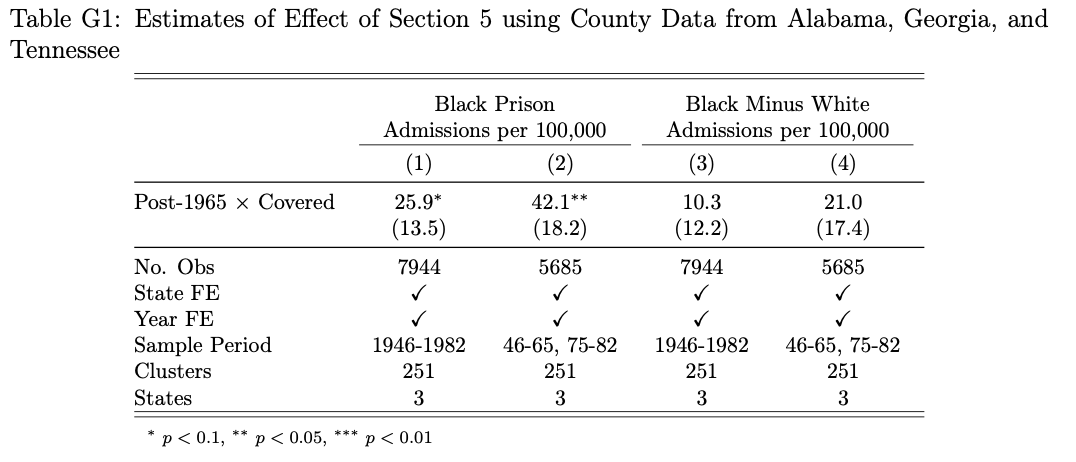
\includegraphics[width=\textwidth]{../../60_appendix_cty_results/table_g1.png}
\end{figure}


\begin{figure}
	\centering
	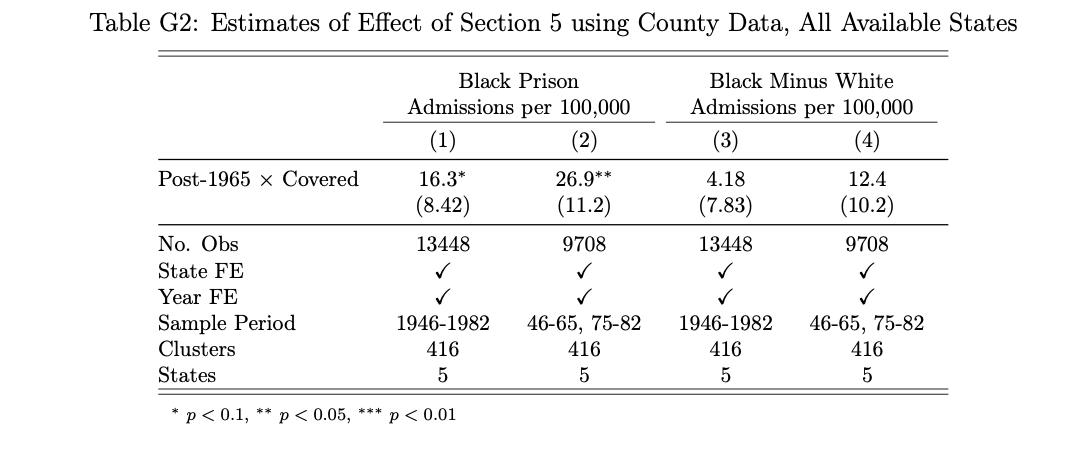
\includegraphics[width=\textwidth]{../../60_appendix_cty_results/table_g2.png}
\end{figure}

% \begin{table}[h!]\centering \footnotesize
% \def\sym#1{\ifmmode^{#1}\else\(^{#1}\)\fi}
% 	\smallskip
% 	\begin{tabular}{@{\extracolsep{5pt}}l*{5}{c}}
% 	\noalign{\smallskip}\hline\hline\noalign{\smallskip}\noalign{\smallskip}
% 			&  \multicolumn{2}{c}{Black Prison }  & \multicolumn{2}{c}{Black Minus White}  \\
% 			&  \multicolumn{2}{c}{Admissions per 100,000} & \multicolumn{2}{c}{Admissions per 100,000}  \\
% 			\cline{2-3} \cline{4-5}   \noalign{\smallskip}
% 				                &\multicolumn{1}{c}{(1)}         &\multicolumn{1}{c}{(2)}         &\multicolumn{1}{c}{(3)}         &\multicolumn{1}{c}{(4)}         \\
\midrule
Post-1965 $\times$ Covered&     25.9\sym{*}  &     42.1\sym{**} &     10.3         &     21.0         \\
                &   (13.5)         &   (18.2)         &   (12.2)         &   (17.4)         \\
\midrule
No. Obs         &     7944         &     5685         &     7944         &     5685         \\
State FE        &\checkmark         &\checkmark         &\checkmark         &\checkmark         \\
Year FE         &\checkmark         &\checkmark         &\checkmark         &\checkmark         \\
Sample Period   &1946-82         &46-65, 75-82         &1946-82         &46-65, 75-82         \\
Clusters        &      251         &      251         &      251         &      251         \\
States          &        3         &        3         &        3         &        3         \\
 \\
% 	\noalign{\vspace*{-.17in}}\hline\hline\noalign{\smallskip}
% \multicolumn{5}{l}{\scriptsize \sym{*} \(p<0.1\), \sym{**} \(p<0.05\), \sym{***} \(p<0.01\)}\\
% \end{tabular}
% \end{table}


% \begin{table}[h!]\centering \footnotesize
% \def\sym#1{\ifmmode^{#1}\else\(^{#1}\)\fi}
% 	\caption{Estimates of Effect of Section 5 using County Data, All Available States}\label{table_county_allstates}
% 	\smallskip
% 	\begin{tabular}{@{\extracolsep{5pt}}l*{5}{c}}
% 	\noalign{\smallskip}\hline\hline\noalign{\smallskip}\noalign{\smallskip}
% 			&  \multicolumn{2}{c}{Black Prison }  & \multicolumn{2}{c}{Black Minus White}  \\
% 			&  \multicolumn{2}{c}{Admissions per 100,000} & \multicolumn{2}{c}{Admissions per 100,000}  \\
% 			\cline{2-3} \cline{4-5}   \noalign{\smallskip}
% 				                &\multicolumn{1}{c}{(1)}         &\multicolumn{1}{c}{(2)}         &\multicolumn{1}{c}{(3)}         &\multicolumn{1}{c}{(4)}         \\
\midrule
Post-1965 $\times$ Covered&     16.3\sym{*}         &    26.9\sym{**} &     4.18         &     12.4         \\
                &   (8.42)         &   (11.2)         &   (7.83)         &   (10.2)         \\
\midrule
No. Obs         &    13448         &     9708         &    13448         &     9708         \\
State FE        &\checkmark         &\checkmark         &\checkmark         &\checkmark         \\
Year FE         &\checkmark         &\checkmark         &\checkmark         &\checkmark         \\
Sample Period   &1946-82         &46-65, 75-82         &1946-82         &46-65, 75-82         \\
Clusters        &      416         &      416         &      416         &      416         \\
States          &        5         &        5         &        5         &        5         \\
 \\
% 	\noalign{\vspace*{-.17in}}\hline\hline\noalign{\smallskip}
% \multicolumn{5}{l}{\scriptsize \sym{*} \(p<0.1\), \sym{**} \(p<0.05\), \sym{***} \(p<0.01\)}\\
% \end{tabular}
% \end{table}


\vspace*{.1in}
\textbf{Heterogeneity by Black Population, All States with County Data}



\begin{figure}
	\centering
	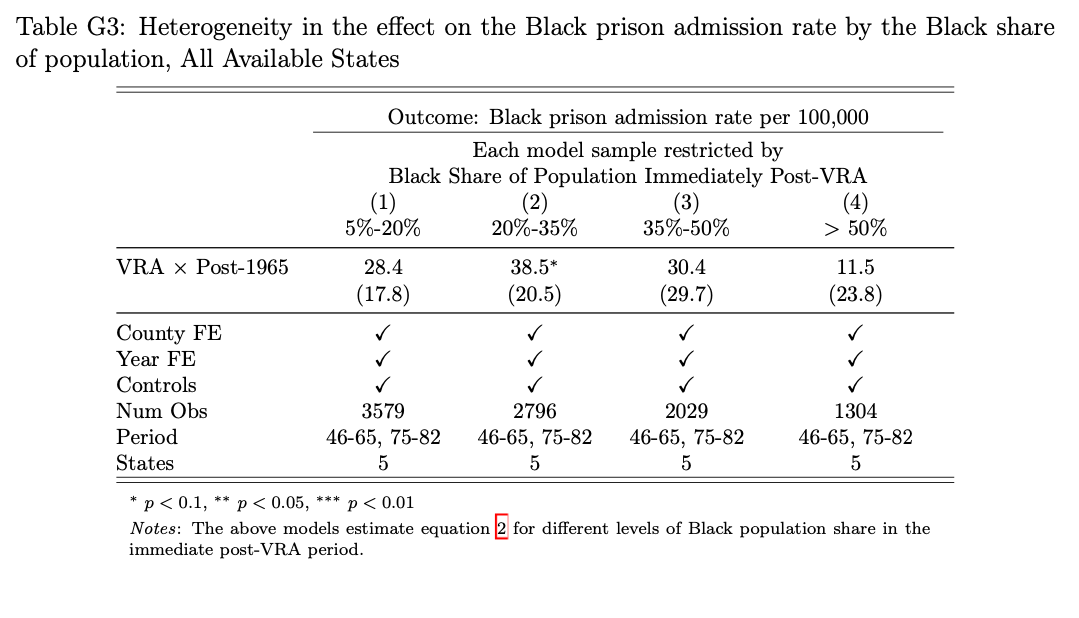
\includegraphics[width=\textwidth]{../../60_appendix_cty_results/table_g3.png}
\end{figure}


\begin{figure}
	\centering
	\includegraphics[width=\textwidth]{../../60_appendix_cty_results/table_g4.png}
\end{figure}
% % TABLE: Heterogeneity black voters Black admissions
% %---------------------------------------------------
% \begin{table}[h!]\centering \footnotesize
% \def\sym#1{\ifmmode^{#1}\else\(^{#1}\)\fi}
% 	\caption{Heterogeneity in the effect on the Black prison admission rate by the Black share of population, All Available States}\label{table_countyheterogeneity_allstates_black}
% 	\smallskip
% 	\begin{tabular}{@{\extracolsep{5pt}}l*{5}{c}}
% 			\noalign{\smallskip}\hline\hline\noalign{\smallskip}\noalign{\smallskip}
% 					&  \multicolumn{4}{c}{Outcome: Black prison admission rate per 100,000} \\
% 					\cline{2-5}   \noalign{\smallskip}
% 					&  \multicolumn{4}{c}{Each model sample restricted by} \\
% 					&  \multicolumn{4}{c}{Black Share of Population Immediately Post-VRA} \\
% 					                &\multicolumn{1}{c}{(1)}&\multicolumn{1}{c}{(2)}&\multicolumn{1}{c}{(3)}&\multicolumn{1}{c}{(4)}\\
                &\multicolumn{1}{c}{5\%-20\%}&\multicolumn{1}{c}{20\%-35\%}&\multicolumn{1}{c}{35\%-50\%}&\multicolumn{1}{c}{$>$ 50\%}\\
\midrule
VRA $\times$ Post-1965&     28.4         &     38.5\sym{*}  &     30.4         &     11.5        \\
                &   (17.8)         &   (20.5)         &   (29.7)         &   (23.8)         \\
\midrule
County FE       &\checkmark         &\checkmark         &\checkmark         &\checkmark         \\
Year FE         &\checkmark         &\checkmark         &\checkmark         &\checkmark         \\
Controls        &\checkmark         &\checkmark         &\checkmark         &\checkmark         \\
Num Obs         &     3579         &     2796         &     2029         &     1304         \\
Period          &46-65, 75-82         &46-65, 75-82         &46-65, 75-82         &46-65, 75-82         \\
States          &        5         &        5         &        5         &        5         \\
 \\
% 	\noalign{\vspace*{-.17in}}\hline\hline\noalign{\smallskip}
% 		\multicolumn{5}{l}{\scriptsize \sym{*} \(p<0.1\), \sym{**} \(p<0.05\), \sym{***} \(p<0.01\)}\\
% 		\multicolumn{5}{p{5.1in}}{\scriptsize  \emph{Notes}: The above models estimate equation~\ref{equation_dind_np} for different levels of Black population share in the immediate post-VRA period. }
% \end{tabular}
% \end{table}





% % TABLE: Heterogeneity black voters Black admissions
% %---------------------------------------------------
% \begin{table}[h!]\centering \footnotesize
% \def\sym#1{\ifmmode^{#1}\else\(^{#1}\)\fi}
% 	\caption{Heterogeneity in the effect on the Black minus White prison admission rate by the Black share of population, All Available States}\label{table_countyheterogeneity_allstates_bminusw}
% 	\smallskip
% 	\begin{tabular}{@{\extracolsep{5pt}}l*{5}{c}}
% 			\noalign{\smallskip}\hline\hline\noalign{\smallskip}\noalign{\smallskip}
% 					&  \multicolumn{4}{c}{Outcome: Black minus White prison admission rates per 100,000} \\
% 					\cline{2-5}   \noalign{\smallskip}
% 					&  \multicolumn{4}{c}{Each model sample restricted by} \\
% 					&  \multicolumn{4}{c}{Black Share of Population Immediately Post-VRA} \\
% 					                &\multicolumn{1}{c}{(1)}&\multicolumn{1}{c}{(2)}&\multicolumn{1}{c}{(3)}&\multicolumn{1}{c}{(4)}\\
                &\multicolumn{1}{c}{5\%-20\%}&\multicolumn{1}{c}{20\%-35\%}&\multicolumn{1}{c}{35\%-50\%}&\multicolumn{1}{c}{$>$ 50\%}\\
\midrule
VRA $\times$ Post-1965&     18.6         &     7.95         &     26.9         &    -2.50         \\
                &   (17.4)         &   (15.2)         &   (39.8)         &   (30.9)         \\
\midrule
County FE       &\checkmark         &\checkmark         &\checkmark         &\checkmark         \\
Year FE         &\checkmark         &\checkmark         &\checkmark         &\checkmark         \\
Controls        &\checkmark         &\checkmark         &\checkmark         &\checkmark         \\
Num Obs         &     3336         &     2662         &     1874         &     1229         \\
Period          &46-65, 75-82         &46-65, 75-82         &46-65, 75-82         &46-65, 75-82         \\
States          &        5         &        5         &        5         &        5         \\
 \\
% 	\noalign{\vspace*{-.17in}}\hline\hline\noalign{\smallskip}
% 		\multicolumn{5}{l}{\scriptsize \sym{*} \(p<0.1\), \sym{**} \(p<0.05\), \sym{***} \(p<0.01\)}\\
% 		\multicolumn{5}{p{5.1in}}{\scriptsize  \emph{Notes}: The above models estimate equation~\ref{equation_dind_np} for different levels of Black voter registration in the immediate post-VRA period. }
% \end{tabular}
% \end{table}


\vspace*{.1in}
\textbf{Heterogeneity by Black Voter Registration}


\begin{figure}
	\centering
	\includegraphics[width=\textwidth]{../../60_appendix_cty_results/table_g5.png}
\end{figure}


\begin{figure}
	\centering
	\includegraphics[width=\textwidth]{../../60_appendix_cty_results/table_g6.png}
\end{figure}

% % TABLE: Heterogeneity black voters Black admissions
% %---------------------------------------------------
% \begin{table}[h!]\centering \footnotesize
% \def\sym#1{\ifmmode^{#1}\else\(^{#1}\)\fi}
% 	\caption{Heterogeneity in the effect on the Black prison admission rate by the Black Voter Registration}\label{table_countyheterogeneity_reg_black}
% 	\smallskip
% 	\begin{tabular}{@{\extracolsep{5pt}}l*{5}{c}}
% 			\noalign{\smallskip}\hline\hline\noalign{\smallskip}\noalign{\smallskip}
% 					&  \multicolumn{4}{c}{Outcome: Black prison admission rates per 100,000} \\
% 					\cline{2-5}   \noalign{\smallskip}
% 					&  \multicolumn{4}{c}{Each model sample restricted by} \\
% 					&  \multicolumn{4}{c}{Black Share of Registration Immediately Post-VRA} \\
% 					                &\multicolumn{1}{c}{(1)}&\multicolumn{1}{c}{(2)}&\multicolumn{1}{c}{(3)}&\multicolumn{1}{c}{(4)}\\
                &\multicolumn{1}{c}{0\%-10\%}&\multicolumn{1}{c}{10\%-20\%}&\multicolumn{1}{c}{20\%-30\%}&\multicolumn{1}{c}{$>$ 30\%}\\
\midrule
VRA $\times$ Post-1965&     77.6\sym{**} &     74.4\sym{***}&    -3.13         &     1.46         \\
                &   (30.5)         &   (19.1)         &   (24.6)         &   (28.8)         \\
\midrule
County FE       &\checkmark         &\checkmark         &\checkmark         &\checkmark         \\
Year FE         &\checkmark         &\checkmark         &\checkmark         &\checkmark         \\
Controls        &\checkmark         &\checkmark         &\checkmark         &\checkmark         \\
Num Obs         &     1895         &     2777         &     1295         &      758         \\
Period          &46-65, 75-82         &46-65, 75-82         &46-65, 75-82         &46-65, 75-82         \\
States          &        5         &        5         &        5         &        5         \\
 \\
% 	\noalign{\vspace*{-.17in}}\hline\hline\noalign{\smallskip}
% 		\multicolumn{5}{l}{\scriptsize \sym{*} \(p<0.1\), \sym{**} \(p<0.05\), \sym{***} \(p<0.01\)}\\
% 		\multicolumn{5}{p{5.1in}}{\scriptsize  \emph{Notes}: The above models estimate equation~\ref{equation_dind_np} for different levels of Black voter registration in the immediate post-VRA period.  }
% \end{tabular}
% \end{table}



% \begin{table}[hb]\centering \footnotesize
% \def\sym#1{\ifmmode^{#1}\else\(^{#1}\)\fi}
% 	\caption{Heterogeneity in the effect on the Black minus White prison admission rate by the Black share of Registration}\label{table_countyheterogeneity_reg_bminusw}
% 	\smallskip
% 	\begin{tabular}{@{\extracolsep{5pt}}l*{5}{c}}
% 			\noalign{\smallskip}\hline\hline\noalign{\smallskip}\noalign{\smallskip}
% 					&  \multicolumn{4}{c}{Outcome: Black minus White prison admission rates per 100,000} \\
% 					\cline{2-5}   \noalign{\smallskip}
% 					&  \multicolumn{4}{c}{Each model sample restricted by} \\
% 					&  \multicolumn{4}{c}{Black Share of Registration Immediately Post-VRA} \\
% 					                &\multicolumn{1}{c}{(1)}&\multicolumn{1}{c}{(2)}&\multicolumn{1}{c}{(3)}&\multicolumn{1}{c}{(4)}\\
                &\multicolumn{1}{c}{0\%-10\%}&\multicolumn{1}{c}{10\%-20\%}&\multicolumn{1}{c}{20\%-30\%}&\multicolumn{1}{c}{$>$ 30\%}\\
\midrule
VRA $\times$ Post-1965&     55.9\sym{**} &     43.0\sym{***}&    -11.1         &    -27.3         \\
                &   (27.7)         &   (16.5)         &   (27.1)         &   (24.0)         \\
\midrule
County FE       &\checkmark         &\checkmark         &\checkmark         &\checkmark         \\
Year FE         &\checkmark         &\checkmark         &\checkmark         &\checkmark         \\
Controls        &\checkmark         &\checkmark         &\checkmark         &\checkmark         \\
Num Obs         &     1903         &     2789         &     1300         &      766         \\
Period          &46-65, 75-82         &46-65, 75-82         &46-65, 75-82         &46-65, 75-82         \\
States          &        5         &        5         &        5         &        5         \\
 \\
% 	\noalign{\vspace*{-.17in}}\hline\hline\noalign{\smallskip}
% 		\multicolumn{5}{l}{\scriptsize \sym{*} \(p<0.1\), \sym{**} \(p<0.05\), \sym{***} \(p<0.01\)}\\
% 		\multicolumn{5}{p{5.1in}}{\scriptsize  \emph{Notes}: The above models estimate equation~\ref{equation_dind_np} for different levels of Black voter registration in the immediate post-VRA period. }
% \end{tabular}
% \end{table}



%--------------------------- APPENDIX K: BEO --------------------------------%
\section{Black Elected Officials}\label{appendix_beo}
\setcounter{table}{0}
\setcounter{figure}{0}
\renewcommand{\thetable}{H\arabic{table}}
\renewcommand{\thefigure}{H\arabic{figure}}
\normalsize


Black political empowerment can take on a number of forms.  In the paper, we focus on conceptualizing and measuring empowerment in terms of electoral strength---the potential size of the Black electorate at the local level (measured by the Black percentage of the total population), and the observed strength of the Black electorate (measured by the share of total voter registrants who are Black).

Of course, the ability to obtain desired policy outcomes may be a function of more than just electoral strength.  Descriptive representation may substitute for such strength, augment it, or descriptive representation may even prove a \emph{necessary} condition for obtaining policy outcomes \citepsec{Preuhs:2006ww}.  Indeed much of the early work of organizations like the Student Non-Violent Coordinating Committee (SNCC) in the South was predicated \emph{not} on turning Blacks out to vote to induce accountability from White incumbents (or even new White candidates), but securing the election of Black candidates who Black voters could ``trust'' to have their interests at heart \citepsec{Jeffries:2009wq}.

Descriptive representation may matter generally across political offices, and it may play a particularly important role in positions most directly related to the carceral state \citepsec{Saltzstein:1989up}.  Local politicians may play a role in managing carceral budgets; organizing and overseeing carceral bureaucracies; and may even play a role in appointing key law enforcement officers.  Then, more specifically, when elected, Black sheriffs, prosecutors and judges can even more directly shape arrests, charges and sentences.

Thus, in addition to an interest in how our main results are conditioned by the electoral strength of Black communities, we are also interested in how those results are conditioned by the election of Black officials.  We want to know if the \emph{Self Policing} argument can explain the main results in our paper.  As with our other tests, for this to be the case, we are interested in whether, in those instances in which Blacks were \emph{most likely} to be able to translate their policy preferences into policy outcomes, we observe an increase in Black incarceration.  That is, does Black elected officeholding result in increased Black political incarceration.  Such evidence would suggest that enfranchisement allowed Black communities to obtain their desired carceral objectives.  Though, as with the size of the Black electorate, we note that Black officeholding is by no means a guarantee of Black policy efficacy;\footnote{For example, instances in which Black elected officials obtained a minority of elected positions may have appeared as a threat as much as evidence of Black political empowerment. } rather, we consider it the place Black communities are more \emph{likely} to be obtaining their preferences.

% preferences are endogenous; they may be subconsciously shaped by dominant views, or strategically adapted on one issue to obtain other desired outcomes.

To examine this heterogeneity, we digitize and entered data from sixteen years of the \emph{Roster of Black Elected Officials} from 1969-1988 for the 11 states of the former Confederacy.\footnote{The 1977 volume was not published to our knowledge.  We also could not obtain the 1982, 1983, 1985 and 1986 volumes.  Resources limited our ability to collect data from a larger sample of states.}  Other scholars have also fruitfully worked with this data \citepsec{Bernini:2017tv,Aneja:2019uz}. These rosters contain entries for every Black official at the state and local level, including the position that they held, and where they held it.  Because the number of officials in the pre-1965 period is essential to being able to use a difference-in-differences design (as in the main paper), we use data presented in \citesec{Bernini:2017tv} on the count of pre-1965 Black elected officials.\footnote{We look at the map in their paper.}  We make the assumption that these are the only officials during the immediate pre-1965 period.  In our research, we have not come across evidence contrary to that assumption.






% %  FIGURE: BEO
% %-------------------------------------------
 \begin{figure}[h!]
 	\begin{center}
 	\caption{Trends in Black elected officials by type in the South}
 	\small

 		\vspace{.2in}
 			\includegraphics[ width=2.1in, clip=true, trim=0.1in 0in 0.05in 0in ]{../../50_results/plot_beo_AL.pdf}
 			\includegraphics[ width=2.1in, clip=true, trim=0.0in 0in 0.05in 0in  ]{../../50_results/plot_beo_AR.pdf}
 			\includegraphics[ width=2.1in, clip=true, trim=0.1in 0in 0.05in 0in  ]{../../50_results/plot_beo_FL.pdf}\\

       \vspace{.05in}
 			\includegraphics[ width=2.1in, clip=true, trim=0.1in 0in 0.05in 0in ]{../../50_results/plot_beo_GA.pdf}
 			\includegraphics[ width=2.1in, clip=true, trim=0.1in 0in 0.05in 0in  ]{../../50_results/plot_beo_LA.pdf}
      \includegraphics[ width=2.1in, clip=true, trim=0.1in 0in 0.05in 0in  ]{../../50_results/plot_beo_MS.pdf} \\

       \vspace{.05in}
 			\includegraphics[ width=2.1in, clip=true, trim=0.1in 0in 0.1in 0in ]{../../50_results/plot_beo_NC.pdf}
 			\includegraphics[ width=2.1in, clip=true, trim=0.1in 0in 0.05in 0in  ]{../../50_results/plot_beo_SC.pdf}
      \includegraphics[ width=2.1in, clip=true, trim=0.1in 0in 0.05in 0in  ]{../../50_results/plot_beo_TN.pdf} \\

      \vspace{.05in}
 			\includegraphics[ width=2.1in, clip=true, trim=0.1in 0in 0.05in 0in ]{../../50_results/plot_beo_TX.pdf}
 			\includegraphics[ width=2.1in, clip=true, trim=0.1in 0in 0.05in 0in  ]{../../50_results/plot_beo_VA.pdf} \\

      \smallskip\smallskip\smallskip
      \includegraphics[ width=3.75in, clip=true, trim=0.1in 0in 0.0in 0in  ]{../../55_results_other/Legend_Beo.png} \\
       \label{figure_beo_states1}
       \end{center}
  {\singlespacing \scriptsize{\emph{Notes:} Plots present trends in the raw counts (not normalized by the number of elected officials) of Black elected officials by type for the 11 states of the former confederacy.  The trends include the total officials at the state and county level (Black solid line), local political officials (gray dashed line), and local law enforcement officials (gray dotted line) excluding officials involved exclusively in civil law.   Note that the y-axis scales are the same for each plot. \singlespacing}}
 \end{figure} \normalsize



Not all offices were elected in all counties and localities during the period we study.  Many were appointed.  Ideally, we would have systematic information on which positions were elected and which were appointed in order to normalize our measurement of descriptive representation.  A single Black elected politician has a different meaning in a context where only one office is elected as opposed to one with dozens of elected positions.

Lacking such detailed information, we instead use information from the \emph{Census of Governments} on the number of elected positions in 1967 and 1977 \citepsec{Census:1968vw,Census:1978wh}.  We assume that the number of elected positions in 1967 applies to the period before 1967 and up to 1969 when the \emph{Allen} decision was made.  We assume the number of elected positions from 1977 applies from 1970 onwards.  Of course, this is imperfect.  The number of elected officials may have been changing more frequently, and may indeed have been changing in response to Black enfranchisement \citesec{Komisarchik:2018wu}.  But as Komisarchik shows, it was the early period, before Allen, that this strategy of political manipulation was put to its greatest use.  Moreover, we lack data from the pre-1967 period on the number of sub-state elected officials, and thus this strategy is the best available if we wish to normalize any pre-1964 Black elected official counts.\footnote{The 1957 Census of Governments publication on popularly elected officials only includes state totals, not county or municipal totals.}  This normalization also doesn't account for the precise institutional setting when institutions are comprised of multiple equal voting members---e.g. municipal councils.  Thus, even in a case where 50\% of local political officials are Black, those officials may not be distributed such that they form a majority in key policymaking positions (though it makes it more likely that they do). Finally, we are able to construct a measure of the number of county and municipal (i.e. local) elected positions, but the data do not disaggregate to law enforcement officials, specifically, which is of special interest in our study.  Generally, we note that Southern states elected county sheriffs (unlike municipal police chiefs who were more likely to be appointed), and that this was an important position in law enforcement and in maintaining Jim Crow racial domination in the South \citepsec{Falcone:1995tr,Moore:1997vy}.


In Figure~\ref{figure_beo_states1} we present state trends in Black elected officials in the 11 states of the former confederacy.  We present trends in (1) law enforcement officials, both state and local; (2) political officials (e.g. alderman, county commissioners) at the local level; and (3) all officials of all types at both the state and local level.\footnote{Law enforcement includes, among others, sheriffs, constables, judges, prosecutors, and court clerks.  Local refers to county and municipal.  We leave education officials out of the count of political officials.}  The plots present totals, not percentages of elected office.  Almost universally, the plots reveal a monotonic increase in elected officials of all types.  In addition, the plots demonstrate how few elected law enforcement officials are Black.

To more formally evaluate how Black elected officials condition our results, we consider models of the form of our two-way fixed effects specification (equation~\ref{equation_dind_np} in the main paper) and associated long difference specification.  We estimate these models using an additional interaction between an indicator for whether a county has any elected offices held by Blacks at the local level (county and municipal combined).\footnote{We use a dichotomous measure rather than measure the share of local offices held by Black elected officials because nearly all variation is at the extensive margin: only          8.3\unskip\% of county-year observations have \emph{any} Black elected officials.}  We focus on non-education political officials, including law enforcement officials (though, again, we cannot separate out law enforcement officials specifically). We model this relationship, as below, using a dichotomous measure of whether a county has any local Black elected officials.  We also introduce a lag structure on Black elected officials to account for the fact that prison admissions are unlikely to be immediately responsive to a change in political power.

For county $c$ in state $i$ in year $t$ we estimate
\begin{align}
     y_{ict} &=& \alpha_{c} + \gamma_{t} + \nu \text{BEO}_{ict} + \delta (\text{Covered}_{i} \times \text{Post-1965}_{t}) \label{equation_beo} \\
     && + \beta (\text{Covered}_{i} \times \text{Post-1965}_{t} \times \text{BEO}_{ict}) + \psi X_{ict} + \epsilon_{ict}  \nonumber
\end{align}

where our unit ($\alpha$) and year ($\gamma$) fixed effects are as before.  Whether a given county had any Black elected officials (BEO) enter the regression as both an independent regressor and as an interaction with our post-1965 and coverage indicators. Note that we can't also estimate interactions between BEO and the post indicator nor BEO and the coverage indicator because the near absence of Black elected officials prior to 1965 makes these co-linear with the triple interaction term.  Thus, we are effectively estimating the post-1965 difference in outcome between the relationship of Black elected officials to coverage compared to the generalized relationship between Black officials to outcomes in the pre-1965 period.

Note that our sample size is constrained to three states for which we have county-level incarceration data and which approximate our full state-sample main results.  Thus, our sample size is significantly constrained as the treatment of coverage is a state-level phenomenon for these states.


%  \begin{table}[h!]\centering \footnotesize
%  \def\sym#1{\ifmmode^{#1}\else\(^{#1}\)\fi}
%  	\caption{County results for heterogeneity in the effect of Section 5 by local Black elected officials}\label{table_county_beo}
%  	\smallskip
%  	\begin{tabular}{@{\extracolsep{5pt}}l*{5}{c}}
%  	\noalign{\smallskip}\hline\hline\noalign{\smallskip}\noalign{\smallskip}
%  			&  \multicolumn{2}{c}{Black Prison }  & \multicolumn{2}{c}{Black Minus White}    \\
% 			&  \multicolumn{2}{c}{Admissions per 100,000 }  & \multicolumn{2}{c}{Admissions per 100,000}    \\
%  			\cline{2-3} \cline{4-5}   \noalign{\smallskip}
%  				                &\multicolumn{1}{c}{(1)}         &\multicolumn{1}{c}{(2)}         &\multicolumn{1}{c}{(3)}         &\multicolumn{1}{c}{(4)}         \\
\midrule
Post-1965 $\times$ Covered $\times$ BEO (\emph{t-}1)&     36.8\sym{**} &     27.9         &     29.1\sym{*}  &     28.3         \\
                &   (18.3)         &   (24.1)         &   (16.3)         &   (21.8)         \\
Post-1965 $\times$ Covered&     18.2         &     30.6         &     2.57         &     6.95         \\
                &   (17.4)         &   (25.1)         &   (17.0)         &   (24.5)         \\
BEO (\emph{t-}1)&    -32.9\sym{**} &    -22.3         &    -27.0\sym{*}  &    -25.5         \\
                &   (15.1)         &   (21.1)         &   (13.9)         &   (19.8)         \\
\midrule
No. Obs         &     7240         &     5174         &     7240         &     5174         \\
State FE        &\checkmark         &\checkmark         &\checkmark         &\checkmark         \\
Year FE         &\checkmark         &\checkmark         &\checkmark         &\checkmark         \\
Sample Period   &1946-1982         &1946-65, 1975-82         &1946-1982         &1946-65, 1975-82         \\
States          &        3         &        3         &        3         &        3         \\
 \\
%  	\noalign{\vspace*{-.17in}}\hline\hline\noalign{\smallskip}
% 	\multicolumn{5}{p{6.1in}}{\scriptsize Table shows heterogeneity in the estimates of the relationship between Section 5 coverage and prison admissions by the election of Black officials to political office at the local level.  The unit of observation is a county-year.  The three states that comprise the analysis sample are Alabama, Georgia and Tennessee.  Both outcomes are normalized admissions per 100,000.  Models 1 and 3 are two-way fixed effects models.  Models 2 and 4 are our long difference specification.  Models are estimated using OLS and errors are corrected both for imputations and county clustering.  All models include a control for the share of the population living in urban areas. We exclude counties with less than 5\% of their population Black.  } \\
%   \multicolumn{5}{l}{\scriptsize \sym{*} \(p<0.1\), \sym{**} \(p<0.05\), \sym{***}
%   \(p<0.01\)}\\
%  \end{tabular}
%  \end{table}

\begin{figure}[htbp]
	\centering
	\includegraphics[width=\textwidth]{../../60_appendix_cty_results/table_h1.png}
\end{figure}


We present the results (using a one year lag) in Table H1.  Results for other lag structures are similar in magnitude. Columns 1 and 3 present two-way fixed effects models, while columns 2 and 4 present long difference results.

The results indicate that the election of Black officials has a negative effect on Black admissions rates and the difference in between Black and White admissions rates (adding the coefficients on the interaction and the separate BEO regressor).\footnote{When we estimate that simple model excluding the interaction term the coefficient on BEO is negative and statistically different from zero in all models. }  Thus, when Black officials are elected, generally, they do not appear to be increasing race-specific incarceration as would have to be the case for our main results to be explained by the \emph{Self Policing} argument.  Instead, overall they are decreasing incarceration.  Given that there were, in effect, almost no Black elected officials in the pre-1965 period, we can interpret the coefficient on BEO as a post-1965 effect of Black elected officials. In addition to the direct effect of Black elected officials, we're also interested in whether that effect differs under covered states.  In We estimate that in covered states, Black elected officials reduced incarceration less than in uncovered states, but our point estimates remain negative (if insignificant).

Thus, these results do not appear to us consistent with the \emph{Self Policing} argument, and thus we take this as evidence that that argument does not explain our main results.







%---------------------- APPENDIX I: Attitudes --------------------------------%
\section{Attitudes to Crime and the Carceral State}\label{appendix_attitudes}
\setcounter{table}{0}
\setcounter{figure}{0}
\renewcommand{\thetable}{I\arabic{table}}
\renewcommand{\thefigure}{I\arabic{figure}}
\normalsize

In this appendix, we consider the punitive attitudes of Blacks relative to Whites in our attempt to ajudicate whether the \emph{New Jim Crow} argument explains our state-level results, or whether they are explained by \emph{Self-Policing}.


\vspace{.25in}
\textbf{Main Evidence}.

First, we examine Black punitive attitudes (relative to Whites) using pre-1965 survey data from Gallup, and a 1969 survey specifically on male attitudes about violence \citep{Violence1969}.  We describe this data in more detail below.  While we have some concerns about using the latter data from a post-treatment survey, we think the comprehensiveness and nuance of the survey questions offers a compelling case for their use.  As opposed to more general attitudes about crime and criminal justice institutions, we use these surveys to focus on evidence as to whether Blacks were likely to have supported (and therefore \emph{increased}) the use, or harshness of carceral institutions in their own communities \emph{relative to} Whites.

%  FIGURE: Gallup data
%----------------------
\begin{figure}[h!]
 \begin{center}
 \caption{Black and White attitudes to the death penalty pre-1965}
 \smallskip \smallskip
 \small
 			(a) Average responses by race  \hspace*{1.2in} (b) Difference in means \\

			\includegraphics[width=3.0in,  clip=true,  trim= 0.0in 0.0in 0.0in 0.0in]{../../50_results/Attitudes_Gallup1.pdf}
			\includegraphics[width=3.0in,  clip=true,  trim= 0.0in 0.0in 0.0in 0.0in]{../../50_results/Attitudes_Gallup2.pdf} \\
			\label{figure_attitudes1}
			 \end{center}
{\scriptsize{\emph{Source:} Gallup polls 1953, 1956, 1957, 1960 and 1965 from the Roper Center for Public Opinion Research.  }} \\
{\scriptsize{\emph{Notes:} Plot (a) above presents average responses to the question ``Do you support the death penalty for persons convicted of murder?'' for each Black and White respondents from five surveys fielded prior to the VRA.  Plot (b) presents the difference in means between Black and White respondents from a simple OLS regression with 95\% confidence intervals.  Points below the dashed line represent years when White attitudes were more punitive than Black attitudes. See below for more details. \singlespacing }}
			\end{figure} \normalsize




Figure~\ref{figure_attitudes1} plots the raw averages and difference in means by race from five years of Gallup polls which ask about support for the death penalty, a key punitive policy for which pre-1965 data is available.  In all years, we estimate that Blacks are less punitive than White respondents, and there is no general trend that suggests Black and White attitudes were differentially changing.

Figure~\ref{figure_attitudes2} plots the Black minus White difference to ten survey questions and five indexes from \cite{Violence1969}.  Crucially, Black respondents were \emph{less} likely than Whites to say that the police should have more power---or that the criminal justice system \emph{in general} needed more power---and \emph{more} likely than Whites to say that police were too powerful.  Blacks were also less likely to say that courts were too lenient, or that the courts had made it too difficult to punish criminals; they had lower scores on the survey's retributiveness index; and they also preferred that the state use \emph{less} ``violence'' against gangs.  On average, therefore, the evidence suggests that at the time of the VRA's passage, Blacks did not prefer a more punitive carceral state relative to Whites in a way that would explain the main results in the paper.

These differences are compelling, but they may obscure class-related differences fundamental to the \emph{Self-Policing} theory.  Although average Black attitudes appear consistently less punitive than Whites---suggesting that the addition of Black voters to the electorate would have resulted in a shift of the median voter towards \emph{less} punitive policy---it may have been the case that a politically pivotal subset of the Black community held more punitive attitudes than the average Black respondent.  Indeed, past work suggests that there may indeed have been such a division --- along class lines --- in the Black community \citep{Fortner:2015uz,FormanJr:2017tz,Clegg:2018uq}.

We investigate this possibility using the same survey data.  In the Gallup data, we do not have access to income measures for the pre-1965 surveys.  Thus, we must approximate class with education.  Given the sample size, we dichotomize education at the (approximate) top quartile.  Our measure of highly educated takes on a value of 1 for respondents with some college or more.

Despite the class divisions predicted by the \emph{Self-Policing} argument, we do not find that elite/middle class Blacks (measured here as more educated respondents) are more likely to support punitive policy as measured by support for the death penalty.  If anything, we find that more highly educated Black respondents are \emph{less} supportive of the death penalty.  We present these estimates for the difference in means in Figure~\ref{figure_attitudes_gallup2} plot (a).  Because of that, we also show in plot (b) that in most years more highly educated Black respondents were less supportive of the death penalty than White respondents.


%  FIGURE: Gallup data 2
%----------------------
\begin{figure}[h!]
 \begin{center}
 \caption{Difference between race and class in support for the death penalty pre-1965}
 \smallskip \smallskip
 \small
		(a) Difference between higher and   \hspace*{1.2in} (b) Difference between higher educated \\
		lower educated Black respondents \hspace*{1.2in}  Black respondents and Whites \\

			\includegraphics[width=3.0in,  clip=true,  trim= 0.0in 0.0in 0.0in 0.0in]{../../50_results/Attitudes_Gallup2_educ.pdf}
			\includegraphics[width=3.0in,  clip=true,  trim= 0.0in 0.0in 0.0in 0.0in]{../../50_results/Attitudes_Gallup3_educ.pdf}
			\label{figure_attitudes_gallup2}
			 \end{center}
{\scriptsize{\emph{Source:} Gallup polls 1953, 1956, 1957, 1960 and 1965 from the Roper Center for Public Opinion Research.  }} \\
{\scriptsize{\emph{Notes:} The above plot (1) shows the difference in means between higher and lower educated Black respondents from a simple OLS regression with 95\% confidence intervals.  Points below the dashed line represent years when more highly educated Black respondents had less punitive preferences. The above plot (b) shows the difference in means between higher educated Black respondents and White respondents also using OLS with 95\% confidence intervals.  Points below the dashed line represent years when more highly educated Black respondents had less punitive preferences than White respondents.  See the text for more details. \singlespacing }}
			\end{figure} \normalsize


In the case of the \cite{Violence1969} data, we define class using both income and education.  Given the sample size we dichotomize each at the (approximate) top quartile. Thus, our measure of upper income takes on a value of 1 for respondents with annual household incomes larger than or equal to \$10,000, while our measure of higher education takes on a value of 1 for respondents with education greater than or equal to some college.  We then estimate separate OLS regressions (for the income measure and the education measure) of difference in means on the sample of Black respondents only.  We note that are 303 Black respondents in our data (53 with a value of 1 on the income measure, and 56 with a value of 1 on the education measure).







%  FIGURE: Punitive attitudes for black and white
%-------------------------------------------
\begin{figure}[h!]
 \begin{center}
 \caption{Difference between Black and White attitudes towards the carceral state, 1969}
 \small
		 \includegraphics[ width=5.9in, clip=true, trim=0.35in 0in 0.0in 0in ]{../../50_results/Attitudes_violence1969_1.pdf}
 \label{figure_attitudes_class}
 	\end{center}
 	{\scriptsize{\emph{Source:} \cite{Violence1969}. }} \\
	{\scriptsize{\emph{Notes:} The survey was fielded on a nationally-representative sample of 1,400 adult males in 1969, including an over-sample of Black people.  Point estimates are OLS estimates of difference in means between Black and White respondents with 95\% confidence intervals.  See text for more details. Estimates use the provided survey weights. \singlespacing }}
\end{figure} \normalsize


We present the results in Figure~\ref{figure_attitudes2}. Across these regressions, we find only four statistically significant differences by class\footnote{Although as we have not implemented any multiple-test corrections, even these should be interpreted with caution.}: upper class Black respondents appear to be slightly more likely to believe ``Police can be trusted,'' slightly less likely to believe ``Police more likely to be victims of crime than cause crime themselves,'' and for one of our two measures of class, slightly more likely to believe ``Courts are too lenient'' but slightly less likely to believe ``Police should have more power.''

Nevertheless, the evidence does not paint a consistent picture of upper class Black respondents supporting more punitive policies. Black respondents with more education were much less likely than less educated Black respondents to support retributive punishment (as measured by the retributiveness index), and less likely to say that the police should have more power.  In addition, upper class Black respondents were nearly statistically significantly more likely to think that the police were too powerful (income only), and less likely to think that the police were victims of crime rather than causes of it (income and education).  We note that many point estimates are extremely close to zero and/or have large confidence intervals suggesting that there were not class differences in terms of responses to those questions, or that there is too much noise to be able to reject the null hypothesis of no class differences.


%  FIGURE: Punitive attitudes for black and white
%------------------------------------------------
\begin{figure}[h!]
 \begin{center}
 \caption{Difference between upper and lower class attitudes towards the carceral state amongst Black respondents only, 1969}
 \small
		 \includegraphics[ width=5.9in, clip=true, trim=0.35in 0in 0.0in 0in ]{../../50_results/Attitudes_violence1969_3.pdf}
 \label{figure_attitudes2}
 	\end{center}
 	{\scriptsize{\emph{Source:} \cite{Violence1969}. }} \\
	{\scriptsize{\emph{Notes:} The above are estimated from the sample of 303 Black respondents.  Black point estimates are OLS estimates of difference in means between upper (>=\$10,000 annual household) and lower income respondents with 95\% confidence intervals. Gray diamond point estimates are OLS estimates of difference in means between high education (>= some college) and lower education respondents.  Estimates are made from separate regressions.  See text for more details.  Estimates use the provided survey weights.  \singlespacing }}
\end{figure} \normalsize

Although the evidence for upper class Black respondents having more punitive attitudes, we proceed with evaluating whether elite/middle class Black respondents (here as measured only by income, which gave the strongest indication of class differences) held punitive preferences that were different from average \emph{White} preferences.  To do that, we restrict our sample to only upper income Black respondents and use OLS to estimate a difference in means relative to all White respondents.  We present the results in Figure~\ref{figure_attitudes_class2}.  We note the similarity in the sign and magnitude between the mean differences in Figures\ref{figure_attitudes1} and~\ref{figure_attitudes_class2}.  The differences in most cases are slightly attenuated towards zero, but the general pattern remains---Black upper income respondents were more likely to think the police should not have more power, that the police were too powerful, to prefer less retributiveness, and to disagree that the courts were too lenient or had made it too difficult to punish criminals.




%  FIGURE: Punitive attitudes for black and white
%-------------------------------------------
\begin{figure}[h!]
 \begin{center}
 \caption{Difference between Black upper income and White attitudes towards the carceral state, 1969}
 \small
		 \includegraphics[ width=5.9in, clip=true, trim=0.35in 0in 0.0in 0in ]{../../50_results/Attitudes_violence1969_4.pdf}
 \label{figure_attitudes_class2}
 	\end{center}
 	{\scriptsize{\emph{Source:} \cite{Violence1969}. }} \\
	{\scriptsize{\emph{Notes:} The survey was fielded on a nationally-representative sample of 1,400 adult males in 1969, including an over-sample of Black people.  The upper income Black respondents included in the sample were 53.   Point estimates are OLS estimates of difference in means between upper class Black respondents (as defined by income) and White respondents with 95\% confidence intervals.  See text for more details.  Estimates use the provided survey weights.  \singlespacing }}
\end{figure} \normalsize


Finally, we also consider whether Black attitudes towards drug crime in particular might be different from other crime.  If Blacks preferred more punitive policies related to drug crimes, and if drug crimes were sufficiently prevalent, these preferences of the electorate could drive growth in incarceration even if the punitive preferences of Blacks for other crimes were less than Whites.  We use data from a 1969 Gallup survey, the first to ask about drugs, which helpfully compares preferred sentence lengths for ``dope peddling'' and five other crimes.  We present the results in Figure~\ref{figure_dope}. Our results document that, if anything, Black respondents preferred shorter sentences for those who sold drugs, not longer sentences.  Finally, when we undertake that same comparison between White and elite/middle-class Black respondents only.  We use a dichotomous measure of income, coding upper income equal to 1 at the top quartile of the income distribution (\$>7,000 annual household income).  Of particular interest is the point estimate on ``dope peddling'' which attenuates to zero, but remains negative and is highly statistically insignificant.  The results comparing elite/middle-class Blacks to Whites can be found in Figure~\ref{figure_dope2}.

Given this evidence, it is difficult to infer that, at the time of the VRA's passage, elite and middle-class Blacks preferred a more punitive carceral state relative to Whites in a way that would have shifted the preferences of the median voter towards more punitive policy.  Instead, we think that this evidence supports interpreting our results as deriving from the \emph{New Jim Crow} argument rather than the \emph{Self-Policing} argument.



%  FIGURE: Punitive attitudes for black and white
%-------------------------------------------
\begin{figure}[h!]
 \begin{center}
 \caption{Difference between Black and White preferred sentence length by crime, 1969}
 \small
		 \includegraphics[ width=4.2in, clip=true, trim=0.35in 0in 0.0in 0in ]{../../50_results/Attitudes_Drugs_black.pdf}
 \label{figure_dope}
 	\end{center}
 	{\scriptsize{\emph{Source:} Gallup poll from 1969 from the Roper Center for Public Opinion Research. }} \\
	{\scriptsize{\emph{Notes:} The above presents difference in means estimated via OLS between Black and White respondents.  Estimates to the right of the dashed line indicate crimes for which, on average, Black respondents referred longer sentence to White respondents.  \singlespacing }}
\end{figure} \normalsize



%  FIGURE: Punitive attitudes for black and white
%-------------------------------------------
\begin{figure}[h!]
 \begin{center}
 \caption{Difference between Upper Class Black and White preferred sentence length by crime, 1969}
 \small
		 \includegraphics[ width=4.2in, clip=true, trim=0.35in 0in 0.0in 0in ]{../../50_results/Attitudes_Drugs_blackclass.pdf}
 \label{figure_dope2}
 	\end{center}
 	{\scriptsize{\emph{Source:} Gallup poll from 1969 from the Roper Center for Public Opinion Research. }} \\
	{\scriptsize{\emph{Notes:} The above presents difference in means estimated via OLS between Black and White respondents.  Estimates to the right of the dashed line indicate crimes for which, on average, upper class Black respondents as measured by income preferred longer sentence to White respondents.  \singlespacing }}
\end{figure} \normalsize



\vspace{.25in}
\emph{Gallup Data}.

We use Gallup data from five surveys fielded in the immediate pre-1965 period: 1953 (No. 522), 1956 (No. 562), 1957 (No. 588), 1960 (No. 625) and 1965 (No. 704).  Note that the 1965 survey was fielded in January, well before the passage of the VRA.  The sample sizes for each survey are: 1498, 2000, 1528, 2999, and 3492.  We use the weighted number of observations, when available.  We obtained the data from the Roper Center for Public Opinion Research.

We focus on the sole punitive policy-related question that we can identify consistently in the data.  The question is also consistently worded through the period.  Note: Column location of the responses vary by survey.

\vspace{.1in}
\begin{shift}
	\vspace{.05in}
	\texttt{Are you in favor of the death penalty for persons convicted of murder? }

\end{shift}

We recode no=0, yes=1 and recode ``somewhat'' responses into that simple binary categorization.  We remove ambiguous and non-responses.  We code the race variable focusing only on Black and White respondents in cases where other races codings are provided.

We also use data from a 1969 Gallup survey (No. 773) that asks about preferred punishments for different crimes including dope peddling, arson, passing a bad check, rape, armed robbery and car theft.  We code the race variable as described above.  We remove psychiatric care, circumstance dependence, and other responses of uncertainty and focus on categories for the sentence length with the maximum being the death penalty.




\vspace{.25in}
\emph{Blumenthal et. al. Data.}

This data is from \citesec{Violence1969}.  The data is a survey of 1,400 adult males in the US in 1969, including an oversample of Black males.\footnote{We used the associated survey weights to adjust for the sampling procedure.}  We examined fifteen questions, some of which were index variables comprised of other variables that we don't present.

	 \vspace{.1in}
	 \begin{shift}
		 \vspace{.05in}
		 \texttt{\textbf{VAR 0043 R1/R2.}}

		 \texttt{What violent events in the United States are of the most concern to you? }


		 \vspace{.05in}
 		\texttt{\textbf{VAR 0098.}}

 		\texttt{Do you think Negroes (Black people/Colored people) are more likely to cause violence, or more likely to be victims of violence, or are they likely to nto be involved?}


 		\vspace{.05in}
 		\texttt{\textbf{VAR 0099.}}

 		\texttt{Do you think Police are more likely to cause violence, or more likely to be victims of violence, or are they likely to not be involved?}

 		\vspace{.05in}
 		\texttt{\textbf{VAR 0137.}}

 		\texttt{On the whole, would you say that most policemen are trying to be helpful, or that they are looking for trouble, or they aren't one way or the other?}

 		\vspace{.05in}
 		\texttt{\textbf{VAR 0138.}}

 		\texttt{Think of how policemen think of people like yourself.  Do you think that none dislike people like yourself, only a few, many or almost all dislike people like yourself?}

 		\vspace{.05in}
 		\texttt{\textbf{VAR 0139.}}

 		\texttt{Would you say that most policemen can be trusted or that you can't be too careful in dealing with them?}

		\vspace{.05in}
 		\texttt{\textbf{VAR 0162.}}

 		\texttt{Police are getting so much power that the average citizen has to worry.}


		\vspace{.05in}
 		\texttt{\textbf{VAR 0163.}}

 		\texttt{Courts nowadays are much too easy on criminals.}

		\vspace{.05in}
 		\texttt{\textbf{VAR 0164.}}

 		\texttt{Recent supreme court decisions have made it more difficult to punish criminals.}


		\vspace{.05in}
		\texttt{\textbf{VAR 0165.}}

		\texttt{Police nowadays should have more power (authority) to enforce the law adequately.}

	 	\vspace{.05in}
		\texttt{\textbf{VAR 0269.}}

		\texttt{Index: Are Police Actions Violence?  A composite score derived from Ref. Nos. 0052, 0053, and 0059. VAR 0052: Do you think of police beating students as violence?  VAR 0053: Do you think of police shooting looters as violence?  VAR 0059: Do you think of police stopping to frisk people as violence?}


		\vspace{.05in}
		\texttt{\textbf{VAR 0273.}}

		\texttt{Index: Retributive Justice Index.  A composite score derived from Ref. Nos. 0148, 0149, 0151, 0152, and 0154.  VAR0148: People who commit murder deserve capital punishment.  VAR 0149: Violence deserves violence.  VAR0151: `An eye for an eye and a tooth for a tooth' is a good rule for living.  VAR0152: It is often necessary to use violence to prevent violence.  VAR0154: When someone does wrong, he should be paid back for it. }

		\vspace{.05in}
		\texttt{\textbf{VAR 0278.}}

		\texttt{Index: Police/Court Power Index.  A one digit index recoded from Ref. Nos. 0163, 0164, 0165.  See those above. }


		\vspace{.05in}
		\texttt{\textbf{VAR 0279.}}

		\texttt{Index: Court Fairness Index.  A one digit index recoded from Ref. Nos. 0133, 0135, 0136.  VAR0133: Some people have told us the courts nowadays treat some people better or worse than others.  Do you think that rich people and poor people are likelyt o be treated the same by the courts or not?  VAR0135: Do you think that White people and Negroes (Black people/Colored people)  are likely to be treated the same by the courts or not?  VAR0136: Do you think the courts treat people like yourself better or worse than others, or about the same? }

		\vspace{.05in}
		\texttt{\textbf{VAR 0285.}}

	 	\texttt{Index: Violence for Social Control--Hoodlum Gangs.  A composite score derived from Ref. Nos. 0073--0076. VAR 0073: Police should make arrests without using clubs or guns when gangs of hoodlums terrify people and cause a lot of property damage.  VAR 0074: Police should use clubs, but not guns when gangs of hoodlums terrify people and cause a lot of property damage.  VAR 0075: Police should shoot but not kill when gangs of hoodlums terrify people and cause a lot of property damage.  VAR 0076: The police should shoot to kill when gangs of hoodlums terrify people and cause a lot of property damage. }

	 \end{shift}
	 \vspace{.1in}


We analyze the above questions by dropping ambiguous responses and non-responses.  We then estimate OLS regressions to produce simple difference of means between Black and White respondents.  For VAR 43 we examine the response of 70 only, which indicates that crime is the first or second issue mentioned.


\vspace{.25in}
\textbf{Additional Evidence}.


Additional data sources and details of the above sources are presented below.

\vspace{.25in}
\emph{Almond and Verba Data}.

This data is from \citesec{Almond:1968vt}. The data is a survey of 970 adults in the US interviewed between 1959 and 1960.  We use only the data from the US.  We examine two questions about crime, presented below.


\vspace{.1in}
\begin{shift}

	\texttt{\textbf{VAR 0064.}}

	\texttt{If you had some trouble with the police--a traffic violation maybe, or being accused on minor offense--do you think you would be given equal treatment, that is, would 	you be treated as well as anyone else?}

	\vspace{.05in}
	\texttt{\textbf{VAR 0065.}}

	\texttt{If you explained your point of view to the police, what effect do you think it woud have.  Would they give your point of view serious consideration, would they pay only a little attention, or would they ignore what you had to say?}
\end{shift}
\vspace{.1in}

We recode the response options for 0064 above (0=no; 1=yes) and for 0065 (0=ignore point of view; 1=little attention; 2=serious consideration). We remove uncertain/ambiguous responses and non-responses. Thus, higher values for both responses indicate greater trust in the police.  Our independent variable is the race of the respondent recoded to Black and White.  We estimate an OLS regression to reflect a simple difference in means.  Figure~\ref{figure_almondverba} presents the results.


 %%  FIGURE: Almond and Verba Attitudes
 %%------------------------------------
 \begin{figure}[h!]
   	\begin{center}
   	\caption{The difference in Black-White attitudes towards the police prior to the VRA (Almond and Verba data)}
   		\small \vspace*{.05in}
   		\smallskip
   			\includegraphics[width=2.0in,  clip=true,  trim= 0.0in 0.0in 0.0in 0.0in]{../../50_results/Attitudes_4_AV.pdf} \\
   		\label{figure_almondverba}
   		\end{center}
  	\scriptsize{\emph{Notes:} The above plot presents a difference in means between Black and White responses to two questions about the police fielded between 1969 and 1970. }
   \end{figure} \normalsize


The results indicate the Black respondents are, on average, less likely to believe that the police would provide them equal treatment and less likely to believe that the police would understand their perspective.  Although these questions lack the nuance of those presented in the main text, they are form the pre-1965 period and are thus the least likely to be endogenous to any post-VRA changes.  Although these questions indicate that Black respondents are less trusting of the police, it is difficult to infer from these questions whether Black respondents prefer more punitive police (and carceral institutions, more generally) as a result.  Though Black respondents might prefer more policing if police are neglecting enforcing the law in their communities (interpreting equal treatment to mean equal police presence, arrests and charges, for instance), it might also be the case that these attitudes indicate a preference for less punitive policing if inequality and an inability to understand the perspective of Black citizens represents \emph{over}-punitiveness.





\vspace{.25in}
\emph{ANES Data}.

We also consider data from \citesec{ANES:2020ut}.  This data lacks the detail of other data (see Blumenthal et. al. below) and the pre-1965 time frame as other data (see above).  But it does give us some information about change over time for a consistent question measured as early as 1966.  The survey is fielded on US adults and the sample size varies slightly by year.  There were 1,257 respondents in our 1966 sample.

 %%  FIGURE: ANES Attitudes
 %%------------------------
 \begin{figure}[h!]
   	\begin{center}
   	\caption{Police feeling thermometer responses from the ANES, 1966-1992}
   		\small \vspace*{.05in}
   		\smallskip
			(a) Averages by race \\
   			\includegraphics[width=4.2in,  clip=true,  trim= 0.0in 0.0in 0.0in 0.0in]{../../50_results/Attitudes_anes2.pdf} \\
				(b) Differences in means between Black and White respondents \\
   			\includegraphics[width=4.2in,  clip=true,  trim= 0.0in 0.0in 0.0in 0.0in]{../../50_results/Attitudes_anes3.pdf}\\
   		\label{figure_anes}
   		\end{center}
  	\scriptsize{\emph{Notes:} The above plots the average responses by race (top) and simple difference in means between those races (bottom) for the police feeling thermometer question from the ANES.}
   \end{figure} \normalsize



The ANES has consistently asked a feeling thermometer question about the police (0-100 scale).
We analyze differences in the response to this question by year between Black and White respondents.  We present the results in Figure~\ref{figure_anes}.  The top plot shows the raw averages by race, while the bottom plot presents the simple difference in means (estimated via OLS).

The feeling thermometers are consistently warm for both races.  Both Black and White respondents report averages above 65 for all years.  However, Black responses are on average always lower than White responses.  In addition, Black responses decline faster than White responses through the early 1970s, before finally recovering somewhat.

From our perspective, the most important years are the earliest years---1966 and 1968---the years that are most likely to reflect pre-VRA attitudes towards one important carceral institution (the police).  While noting that we lack the ideal pre-196imputation data, we still don't find compelling evidence that Black voters may have had an affirmative policy preference for more incarceration in their communities.







% %--------------------------- APPENDIX J: Fisher --------------------------------%
\section{Fisher Randomization Tests}\label{appendix_fisher}
\setcounter{table}{0}
\setcounter{figure}{0}
\renewcommand{\thetable}{J\arabic{table}}
\renewcommand{\thefigure}{J\arabic{figure}}
\normalsize

\newcommand{\fisherN}{5000}

In light of recent work illustrating the potential for frequentist techniques to overestimate statistical significance \citep{Young:2019jx}, this appendix presents p-values for the models presented in Table~\ref{table_state} calculated using Fisher Randomization Tests (FRTs) \cite{Fisher:1935uc}.

These are conducted by randomizing state-level assignment to treatment (Section 5 coverage) \fisherN\ times and fitting our models with those randomized treatment assignments. We then record the regression p-values associated with our difference-in-difference coefficient from each draw, and compare the regression p-values generated with true values of Section 5 coverage to the overall distribution of regression p-values generated with random treatment assignment. The relative position of the regression p-value calculated with true assignments within the distribution of all p-values is then used to calculate Fisher p-value. Full regression p-value distributions and Fisher p-values are presented below.

\begin{figure}[bh!]
	\centering
	\caption{Black Incarceration Rates}\label{figure_fisher1}
	\includegraphics[width=0.3\textwidth]{../../50_results/fisher_1_linear_model_\fisherN_ols.pdf}\includegraphics[width=0.3\textwidth]{../../50_results/fisher_1_twoway_FEs_\fisherN_ols.pdf}\includegraphics[width=0.3\textwidth]{../../50_results/fisher_1_long_diff_\fisherN_ols.pdf}
\end{figure}


\begin{figure}[bh!]
	\centering
	\caption{Black Minus White Incarceration Rates}\label{figure_fisher2}
	\includegraphics[width=0.3\textwidth]{../../50_results/fisher_2_linear_model_\fisherN_ols.pdf}\includegraphics[width=0.3\textwidth]{../../50_results/fisher_2_twoway_FEs_\fisherN_ols.pdf}\includegraphics[width=0.3\textwidth]{../../50_results/fisher_2_long_diff_\fisherN_ols.pdf}
\end{figure}


% %--------------------------- APPENDIX J: FGLS --------------------------------%
\section{Feasible Generalized Least Squares Results}\label{appendix_fgls}
\setcounter{table}{0}
\setcounter{figure}{0}
\renewcommand{\thetable}{K\arabic{table}}
\renewcommand{\thefigure}{K\arabic{figure}}
\normalsize

In Table~\ref{table_state_fgls} below, we present results estimated using Feasible GLS. Due to heteroskedasticity across states, FGLS is asymptotically more efficient than OLS \citep{Cameron:2005vy}. However, when we apply Fisher Randomization Tests (Appendix~\ref{appendix_fisher}) to our FGLS model, we find that the regression p-values on our difference-in-difference coefficient are highly non-uniform when we randomly permute treatment assignment. In particular, this diagnostic suggests FGLS is overly likely to reject the null hypothesis of no effect. We interpret this as evidence that at the samples sizes we are working with, FGLS remains biased, and is thus not our preferred estimator.

% TABLE 1: State results
%-------------------------
\begin{table}[t!]\centering \footnotesize
	\def\sym#1{\ifmmode^{#1}\else\(^{#1}\)\fi}
		\caption{State results for Section 5 and the Black admissions rate}\label{table_state_fgls}
		\smallskip
		\begin{tabular}{@{\extracolsep{5pt}}l*{7}{c}}
		\noalign{\smallskip}\hline\hline\noalign{\smallskip}\noalign{\smallskip}
				&  \multicolumn{3}{c}{Black Prison }  & \multicolumn{3}{c}{Black Minus White}  \\
				&  \multicolumn{3}{c}{Admissions per 100,000} & \multicolumn{3}{c}{Admissions per 100,000}  \\
				\cline{2-4} \cline{5-7}   \noalign{\smallskip}
					                &\multicolumn{1}{c}{(1)}         &\multicolumn{1}{c}{(2)}         &\multicolumn{1}{c}{(3)}         &\multicolumn{1}{c}{(4)}         &\multicolumn{1}{c}{(5)}         &\multicolumn{1}{c}{(6)}         \\
\midrule
Post-1965 $\times$ Covered ($\beta$)&     1.60         &     24.2         &     47.4\sym{**} &     0.34         &     19.0         &     41.3\sym{**} \\
                &   (12.8)         &   (17.8)         &   (24.1)         &   (10.3)         &   (13.4)         &   (18.6)         \\
Covered $\times$ \emph{T}&    -0.48         &                  &                  &    -0.72         &                  &                  \\
                &   (0.97)         &                  &                  &   (0.83)         &                  &                  \\
Post-1965 $\times$ \emph{T}&     1.56         &                  &                  &    0.076         &                  &                  \\
                &   (1.92)         &                  &                  &   (1.70)         &                  &                  \\
Post-1965 $\times$ Covered $\times$ \emph{T} ($\omega$)&     4.16\sym{**} &                  &                  &     4.03\sym{**} &                  &                  \\
                &   (1.96)         &                  &                  &   (1.81)         &                  &                  \\
\emph{T}        &     2.53         &                  &                  &     2.05         &                  &                  \\
                &   (1.66)         &                  &                  &   (1.28)         &                  &                  \\
Post-1965       &    -7.66         &                  &                  &     6.28         &                  &                  \\
                &   (6.92)         &                  &                  &   (6.30)         &                  &                  \\
\midrule
Diff-in-Diff, 1980&     64.1         &                  &                  &     60.8         &                  &                  \\
Diff-in-Diff, 1980, pvalue&  0.038**         &                  &                  &  0.030**         &                  &                  \\
No. Obs         &      666         &      666         &      504         &      666         &      666         &      504         \\
State FE        &\checkmark         &\checkmark         &\checkmark         &\checkmark         &\checkmark         &\checkmark         \\
Year FE         &                  &\checkmark         &\checkmark         &                  &\checkmark         &\checkmark         \\
Sample Period   &1946-1982         &1946-1982         &46-65, 75-82         &1946-1982         &1946-1982         &46-65, 75-82         \\
Clusters        &       18         &       18         &       18         &       18         &       18         &       18         \\
 \\
		\noalign{\vspace*{-.17in}}\hline\hline\noalign{\smallskip}
	\multicolumn{7}{p{7.0in}}{\scriptsize Table shows estimates of the impact of Section 5 coverage on two outcomes: Black prison admission rates per 100,000 people (columns 1-3) and the difference between Black and White prison admission rates (columns 4-6). Columns (1) and (4) present our linear-in-time difference-differences including the implied estimate at 1980. Columns (2) and (5) estimate our two-way fixed effects model. Columns (3) and (6) estimate our ``long-difference'' with 1965-1975 dropped to account for the fact states may have been slow to respond to passage of the VRA, causing the effect of the VRA to be under-estimated if these early years of adjustment are included. All models are estimated using FGLS.  Multiple imputation adjustments are made to account for missing data interpolation and associated estimation uncertainty. Errors are also clustered by state. All regressions include a control for share of population living in urban areas.} \\
	\multicolumn{7}{l}{\scriptsize \sym{*} \(p<0.1\), \sym{**} \(p<0.05\), \sym{***} \(p<0.01\)}\\
	\end{tabular}
	\end{table}


% %--------------------------- APPENDIX L: FGLS --------------------------------%
\section{Event Study}\label{appendix_eventstudy}
\setcounter{table}{0}
\setcounter{figure}{0}
\renewcommand{\thetable}{L\arabic{table}}
\renewcommand{\thefigure}{L\arabic{figure}}
\normalsize

In Table~\ref{table_eventstudy} below, we estimate the relationship between Section 5 coverage and Black incarceration separately for different 5-year periods (include 1955-1960 and 1960-1965, during which period we code states as covered by Section if they were later covered). The omitted category is incarceration from 1945-1955.

As expected, there is no evidence of a ``Section 5'' effect prior to 1965. Consistent with the results in Figure~\ref{figure_state_section5}, we also see that the impact of Section 5 on prison admissions was not felt immediately, but rather increased only a small amount from 1965 to 1970 before taking off from 1970 to 1982.

\begin{table}[bh!]\centering \footnotesize
	\def\sym#1{\ifmmode^{#1}\else\(^{#1}\)\fi}
		\caption{Event Study}\label{table_eventstudy}
		\smallskip
		\begin{tabular}{@{\extracolsep{5pt}}l*{3}{c}}
		\noalign{\smallskip}\hline\hline\noalign{\smallskip}\noalign{\smallskip}
				&  \multicolumn{1}{c}{Black Admissions}  & \multicolumn{1}{c}{Black Minus White}  \\
				&  \multicolumn{1}{c}{per 100,000} & \multicolumn{1}{c}{Admissions per 100,000}  \\
				  \noalign{\smallskip}
					                &\multicolumn{1}{c}{(1)}         &\multicolumn{1}{c}{(2)}         \\
\midrule
Sec 5 x 1955-1960&    -5.35         &    -6.09         \\
                &   (9.76)         &   (8.51)         \\
Sec 5 x 1960-1965&    -3.46         &    -7.05         \\
                &   (14.2)         &   (11.2)         \\
Sec 5 x 1965-1970&     12.4         &     6.44         \\
                &   (21.1)         &   (17.2)         \\
Sec 5 x 1970-1975&     36.7         &     27.5         \\
                &   (33.9)         &   (27.1)         \\
Sec 5 x 1975-1982&     59.6         &     50.3\sym{*}  \\
                &   (37.3)         &   (30.0)         \\
\midrule
No. Obs         &      666         &      666         \\
State FE        &\checkmark         &\checkmark         \\
Year FE         &\checkmark         &\checkmark         \\
Clusters        &       18         &       18         \\
 \\
		\noalign{\vspace*{-.17in}}\hline\hline\noalign{\smallskip}
		\multicolumn{3}{p{4.0in}}{\scriptsize  \emph{Notes}: The above models estimate the two-way fixed effect model from equation~\ref{equation_dind_np} with treatment divided into smaller intervals. Omitted category is 1945-1955.} \\
		\multicolumn{3}{l}{\scriptsize \sym{*} \(p<0.1\), \sym{**} \(p<0.05\), \sym{***} \(p<0.01\)}\\

	\end{tabular}
	\end{table}.





% %--------------------------- APPENDIX N: County Heterogeneity, Black Minus White --------------------------------%
\section{County Heterogeneity: Black minus White}\label{appendix_countyheterogeneity_blackminuswhite}
\setcounter{table}{0}
\setcounter{figure}{0}
\renewcommand{\thetable}{M\arabic{table}}
\renewcommand{\thefigure}{M\arabic{figure}}
\normalsize



% TABLE: Heterogeneity black voters Black admissions
%---------------------------------------------------
% \begin{table}[h!]\centering \footnotesize
% 	\def\sym#1{\ifmmode^{#1}\else\(^{#1}\)\fi}
% 		\caption{Heterogeneity in the effect on the Black minus White prison admission rate by the Black share of population}\label{table_heterogeneous2}
% 		\smallskip
% 		\begin{tabular}{@{\extracolsep{5pt}}l*{5}{c}}
% 			\noalign{\smallskip}\hline\hline\noalign{\smallskip}\noalign{\smallskip}
% 						&  \multicolumn{4}{c}{Outcome: Black minus White prison admission rates per 100,000} \\
% 					\cline{2-5}   \noalign{\smallskip}
% 						&  \multicolumn{4}{c}{Each model sample restricted by} \\
% 						&  \multicolumn{4}{c}{Black Share of Population Immediately Post-VRA} \\
% 					                &\multicolumn{1}{c}{(1)}&\multicolumn{1}{c}{(2)}&\multicolumn{1}{c}{(3)}&\multicolumn{1}{c}{(4)}\\
                &\multicolumn{1}{c}{5\%-20\%}&\multicolumn{1}{c}{20\%-35\%}&\multicolumn{1}{c}{35\%-50\%}&\multicolumn{1}{c}{$>$ 50\%}\\
\midrule
VRA $\times$ Post-1965&    4.67         &     56.0         &     55.0 &     30.2         \\
                &   (22.9)         &   (63.8)         &   (36.7)         &   (33.8)         \\
\midrule
County FE       &\checkmark         &\checkmark         &\checkmark         &\checkmark         \\
Year FE         &\checkmark         &\checkmark         &\checkmark         &\checkmark         \\
Controls        &\checkmark         &\checkmark         &\checkmark         &\checkmark         \\
Num Obs         &     1794         &     1635         &     1344         &      912         \\
Period          &46-65, 75-82         &46-65, 75-82         &46-65, 75-82         &46-65, 75-82         \\
States          &        3         &        3         &        3         &        3         \\
 \\
% 		\noalign{\vspace*{-.17in}}\hline\hline\noalign{\smallskip}
% 		\multicolumn{5}{l}{\scriptsize \sym{*} \(p<0.1\), \sym{**} \(p<0.05\), \sym{***} \(p<0.01\)}\\
% 		\multicolumn{5}{p{5.1in}}{\scriptsize  \emph{Notes}: The above models estimate the long difference version of equation~\ref{equation_dind_np} for different levels of Black population in the immediate post-VRA period, dropping the years 1965-1974.  In Appendix~\ref{appendix_county}, we observe similar non-monotonicities using the Black share of registered voters. The cut points are chosen based on the distribution county Black population, with the constraint of one group above 50\%.  We note that only two non-covered counties enter into our sample in model 4.  We include a control for share of the county that is urban.  We exclude counties with less than 5\% of the population Black.}
% 	\end{tabular}
% 	\end{table}
\begin{figure}[bh!]
	\centering
	\includegraphics[width=\textwidth]{../../60_appendix_cty_results/table_m1.png}
\end{figure}

%---------------------- APPENDIX M: Perturbations --------------------------------%
\section{Robustness to Maximally Influence Perturbations}\label{appendix_broderick}
\setcounter{table}{0}
\setcounter{figure}{0}
\renewcommand{\thetable}{N\arabic{table}}
\renewcommand{\thefigure}{N\arabic{figure}}
\normalsize

Table~\ref{table_mip} below presents the minimum number of observations that must be removed from the dataset to change different properties of the long-difference difference-in-difference coefficient (N=504). As the table shows, selectively removing a small number of the most influential observations can push the estimate to being below statistical significance, but the table shows one would need to remove at least 97 (of 504) observations in order to flip the sign of the coefficient of interest, and no amount of data removal could generate a negative statistically significant coefficient.

Note that due to limitations of the \cite{broderick2021} software, these estimates are based on a single draw from our multiple imputation datasets, and thus do not quite accurately account for interpolation uncertainty (though because the dataset is not best-guess interpolations, but rather one of the multiple imputation draws, interpolation uncertainty is being accounted for partially).

% TABLE: Maximally Influential Perturbations
%---------------------------------------------------
\input{../../50_results/maximally_influential_Perturbations_longdiff.tex}



\pagebreak \clearpage


%---------------------- SECTION: SECOND BIBLIOGRAPHY -----------------------------%

\singlespacing
\bibliographystylesec{apsr.bst}
\bibliographysec{EubankFresh_Incarceration_bibliography.bib}




%------------------------------ END OF DOCUMENT ------------------------------------%

\end{document}
